%========================================================================
%   FileName: monocularpedestrian.tex
%     Author: GuanHWang
%      Email: GuanHWang2011@gmail.com
% LastChange: 2014-02-28 14:04:48
%========================================================================
\documentclass[10pt,letterpaper,journal,compsoc]{IEEEtran}
\usepackage[CJKchecksingle,CJKnumber]{xeCJK}
\setCJKmainfont[BoldFont={SimHei},
ItalicFont={KaiTi}]{SimSun}
\renewcommand\baselinestretch{1.2}
\usepackage{graphicx}
\usepackage{fixltx2e}
\usepackage{dblfloatfix}
\usepackage{xcolor}
\usepackage[bookmarksnumbered, pdfencoding=auto, 
breaklinks, colorlinks, linkcolor=blue, urlcolor=black, citecolor=blue]{hyperref}
\usepackage{cite}
\usepackage{amssymb}
\punctstyle{plain}
\begin{document}
%\begin{CJK}{UTF8}{hei}
\title{Monocular Pedestrian Detection:\\Survey and Experiments\\
		单眼视觉行人检测:综述和实验}
\author{Markus Enzweiler,~\IEEEmembership{Student Member,~IEEE,}
        and~Dariu M.~Gavrila
\IEEEcompsocitemizethanks{\IEEEcompsocthanksitem M. Enzweiler is with the Department 
of Mathematics and ComputerScience, Image and Pattern Analysis Group, University of Heidelberg,
Speyerer St. 4, 69115 Heidelberg, Germany.\protect\\
E-mail: uni-heidelberg.enzweiler@daimler.com.
\IEEEcompsocthanksitem D.M. Gavrila is with the Environment Perception Department, Assistance
Systems \& Chassis, Daimler AG Group Research, Wilhelm Runge St. 11,
89081 Ulm, Germany, and the Intelligent Systems Lab, Faculty of Science,
University of Amsterdam, Kruislaan 403, 1098 SJ Amsterdam, The
Netherlands.\protect\\
E-mail: dariu.gavrila@daimler.com.}% <-this % stops a space
\thanks{Manuscript received 18 Jan. 2008; revised 14 July 2008; accepted 8 Oct. 2008;
published online 17 Oct. 2008.\protect\\
Recommended for acceptance by T. Darrell.\protect\\
For information on obtaining reprints of this article, please send e-mail to:
tpami@computer.org, and reference IEEECS Log Number\protect\\
TPAMI-2008-01-0039.\protect\\
Digital Object Identifier no. 10.1109/TPAMI.2008.260.}}

%Headers
\markboth{IEEE TRANSACTIONS ON PATTERN ANALYSIS AND MACHINE INTELLIGENCE,~~Vol.~31,~~No.~12, DECEMBER~2009}%
{ENZWEILER AND GAVRILA: MONOCULAR PEDSTRIAN DETECTION: SURVEY AND EXPERIMENTS}

%ID Mark
\IEEEpubid{0162--8828/09/\$25.00~\copyright~2009 IEEE~~~~~Published by the IEEE Computer Society}

%Abstract
\IEEEtitleabstractindextext{%
\begin{abstract}
行人检测是计算机视觉中快速发展的一个领域,在智能汽车,监控系统和高级机器人等方面
具有关键性应用.这篇文章的目的是同时从方法学和实验学视角提供一个关于(该领域)目   
前的技术发展水平的综述.文章的第一部分是一个概览.这一部分涵盖了行人检测系统的主要
组件和底层模型.文章的第二(同时也是占更大比重的)部分是一个相关的实验研究.我们
考察了目前具有代表性的多种系统模型:基于小波的AdaBoost级联器\cite{bib74},
HOG/linSVM\cite{bib11},NN/LRF\cite{bib75},和联合形状-纹理检测器
\cite{bib23}.实验采用城市环境行驶车辆捕获的泛数据集.数据集包含了多达数以
千计的训练样本以及一个27分钟的包含了超过20,000张具有行人位置注释的
图像的测试序列.我们考察了一般评估设定和车载系统行人检测的特殊评估设定.实验结果
表明HOG/linSVM在高分辨率和低处理速度条件下的明显优势,同时,基于小波的AdaBoost级联器
在较低分辨率和(接近于)实时处理速度条件下的优势.数据集(8.5GB)公诸于众满足
基准测试的目的.
\end{abstract}

%Keywords
\begin{IEEEkeywords}
%Pedestrian detection,survey,perfoemance analysis,benchmarking.\\
行人检测,综述,性能分析,基准测试。
\end{IEEEkeywords}}

\maketitle
\IEEEdisplaynontitleabstractindextext
\section{导言}
对图像进行人体检测是诸多重要应用的一项关键环节.在这篇文章中,
我们只关注那些待检测人体只占图像较小部分的应用设定,即在低分辨
率下的可视对象.这包括了诸多户外设定,例如:摄像头俯视监视街道的监控
系统,车载摄像头监视前方道路的行人以评估潜在碰撞可能性的智能汽车.人
体检测同时也可应用于诸如机器人检测过道上的行人的室内设定.因此本文
剩余部分我们都用``行人''这个词,而不是更泛义的``人''.我们不考察例如
人类姿态复原或是行为识别等更具体的获取任务.

行人检测从机器视觉的角度来说是一项困难的任务.由于显式模型的匮乏,
我们选择使用从实例样本中学习隐式表示的机器学习技术.就其本身而言,行人
检测是多级对象分类问题的一个案例(例如,\cite{bib79}).然而行人检测任务
具有一些自己的特征,这会影响到选择的方法.首先,存在很多可能的行人
外形,依赖于姿势,穿着,光照条件以及背景等因素.检测装置通常是装
配在物理环境中的系统的一部分,这意味着先验知识(相机校正,地平面约束)
能够提升性能.收集泛数据集是相当耗费精力的;这项研究就得益于
已有的数以千计的样本.另一方面,我们将会看到,行人检测对于性能和处理
速度的门槛要相对高出许多.

\begin{figure*}[!t]
\centering
\large{\textbf{TABLE~1\\Overview of Publicly Available Pedestrian Data Sets with Ground-Truth}}
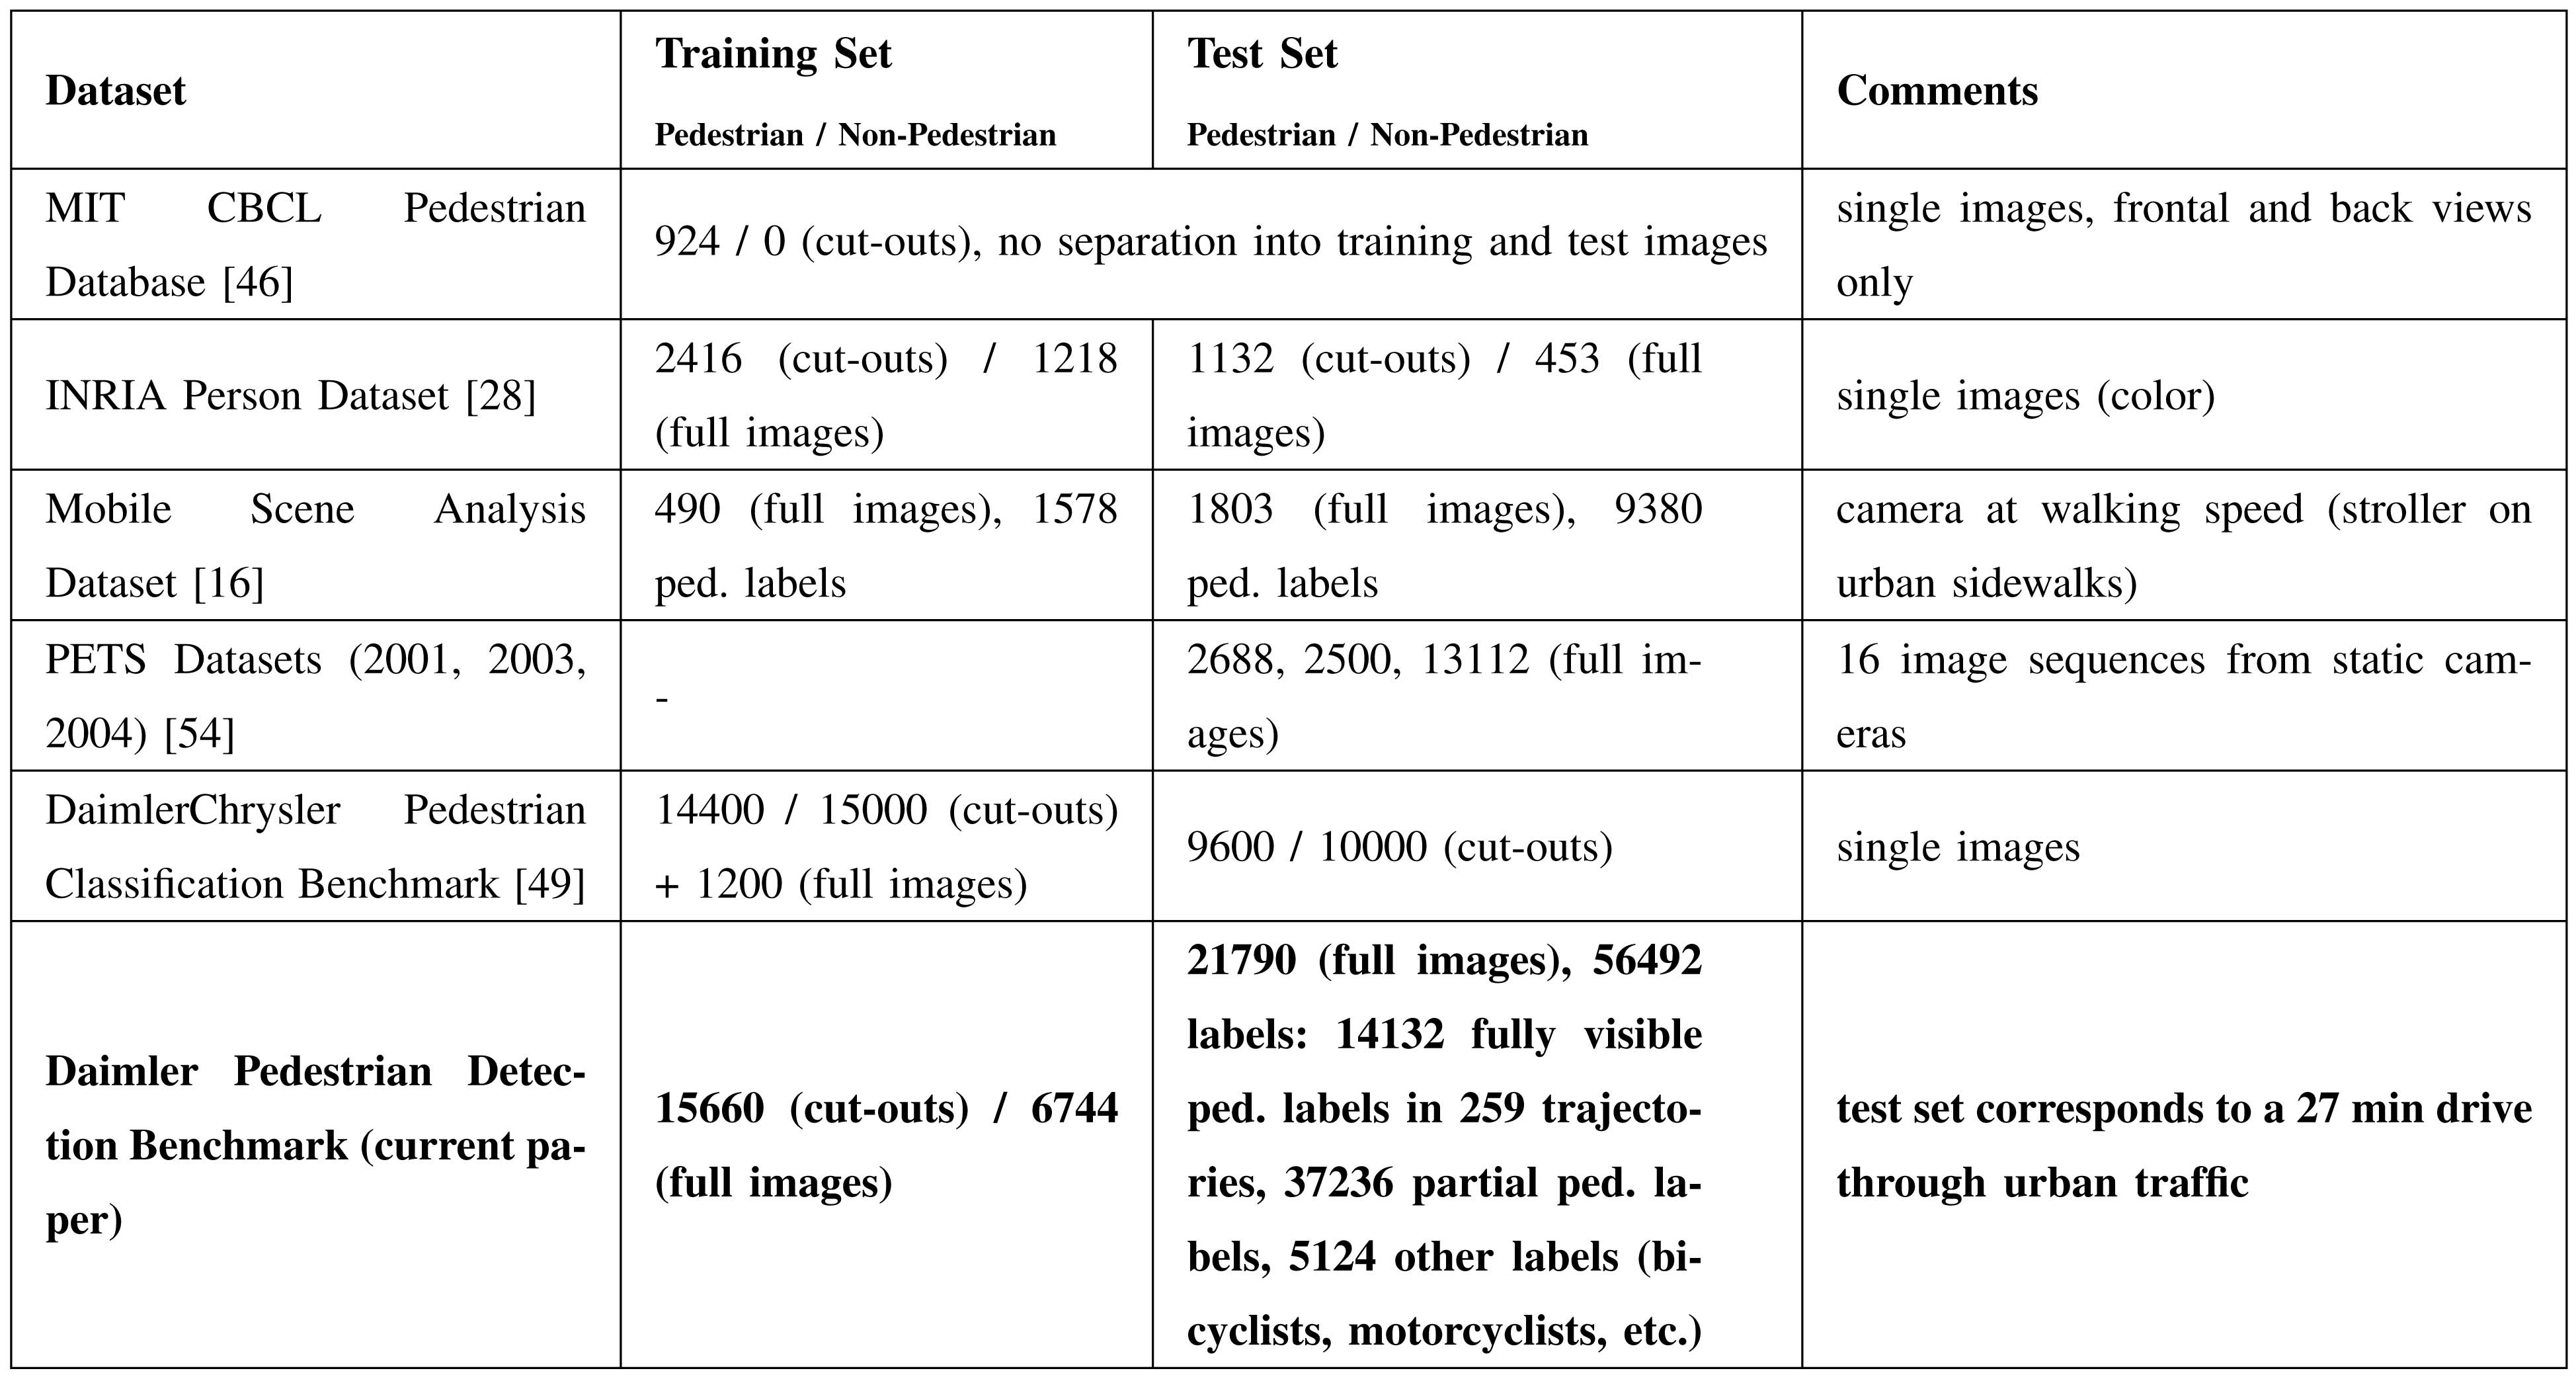
\includegraphics[width=7in]{table1.JPG}
\end{figure*}
行人检测在过去数年内吸引了相当数量的来自计算机视觉社区的研究兴趣.
许多技术理论以特征,模型和泛型架构的形式被提出.然而在实验方面情况并不是
这么乐观.报告中提及的性能往往相差几个数量级(例如,\cite{bib74}内部的
性能差异或\cite{bib39}与\cite{bib74}相比的性能差异).这源于采用的图像数据
的类型差异(背景变化的程度),测试数据集的有限大小,以及不同(通常未被
详细规定)的评估标准:定位容差,覆盖范围等.

这篇文章旨在同时从方法论角度和实验学角度,通过提供一个通用的基准参考
点来提高性能评估的可视化程度.为了达到这个目的,文章的第一部分将会是一个综述,
涵盖了行人检测系统的主要组件:假设生成(ROI选择),分类(模
型匹配),以及目标跟踪.文章第二部分是一个相关的实验研究.我们用之后提及的相
同标准和数据集评估多种具有代表性的系统:
\begin{enumerate}
\item[$\bullet$]基于Haar小波的AdaBoost级联器\cite{bib74};
\item[$\bullet$]方向梯度直方图(HOG)特征与线性支持向量机的组合\cite{bib11};
\item[$\bullet$]采用局部感知域特征的神经网络(NN/LRF) \cite{bib75}; 
\item[$\bullet$]分层形状匹配和基于纹理的NN/LRF分类器的组合\cite{bib23}.
\end{enumerate}

在评估方面,我们同时考察一般测试场景和限定特殊应用的测试场景.
一般测试场景即评估一种行人检测方法的固有潜力.由于一般测试场景
采用一个简单2维边界盒重叠标准用于匹配,不会引入先验知识.此外,
它对可容许处理时间没有任何限制(不考虑实际可行性).限定特殊应用的
测试场景聚焦于车载行人检测系统的应用,在这种测试场景下关于相机
校正,地平面定位以及可感知传感器覆盖范围的信息提供了感兴趣区域(ROI).
评估在涉及车辆的三维坐标系中进行.此外,我们对可容许处理时间设定了
限制(每帧250毫秒与每帧2.5秒).在两种测试场景中,我们都列出了在帧层面和
轨线层面的检测性能.

数据集事实上是相当大规模的;它包括了数以万计的训练样本以及一个
历时27分钟的从城市交通行驶中采集的由21,790张分辨率
为$640\times480$单眼图像的测试序列.如TABLE~1所示.与之前的行人
数据相比,序列图像的存在意味着假设生成和行人检测系统的跟踪组件
同样可以得到评估,而不像\cite{bib28},\cite{bib46},\cite{bib49}那样.
此外,数据集在复杂度(动态变化的背景)和在车载行人碰撞保护应用中的情景真
实性方面表现卓越.

这篇文章的视野相比我们之前的聚焦于用低分辨率($18\times36像素$)
行人和非行人轮廓图像进行行人分类实验研究\cite{bib49}有显著的拓宽.
这里,我们对在一般场景和限定特殊应用(车载)的场景设定下的图像序列
中定位行人的鲁棒性和有效性进行评估.在考察的方法中,我们包括了依赖
于由粗到精的图像搜索策略的方法,例如,见Section~4.4.

文章下文组织如下:第2节对单眼视觉行人检测进行综述.在第3节中
介绍我们的基准测试数据集,之后,第4节描述用于实验评估的方法.一般评估
和限定特殊应用(车载)的评估的结果将在第5节中陈列.在第6节中讨论结果后,
我们在第7节中作出结论.
\section{综述}
虽然与本文的聚焦点有所不同,还是存在许多相关的综述.
\cite{bib21},\cite{bib47},\cite{bib57}的作者报告了人体检测,人体姿式估
计和行为识别的方法.Gandhi和Trivedi
\cite{bib20}聚焦于行人保护在智能汽车领域中的应用.他们同时论述了
被动和主动安全保护技术,后者采用了多视觉和非视觉传感器与碰撞风险评估技术.
我们将行人检测分解为初始对象假设生成(ROI选择),验证(分类),以及时域整合
(跟踪).由于后两者需要行人类模型,例如,形体,外貌或动力学等方面,感兴趣区域
(ROI)的初始生成通常是基于更一般的低级特征或是先验知识.
\subsection{ROI选择}
采用滑窗技术获取初始对象位置假设是最简单的方法,在这种方法中检测窗口
以不同的大小和位置在图像上位移.计算消耗往往会超出实时处理
容限\cite{bib11},\cite{bib12},\cite{bib48},\cite{bib53},\cite{bib60},\cite{bib68}.
通过将滑窗技术与递增复杂度的级联分类器结合\cite{bib45},\cite{bib52},\cite{bib63}
,\cite{bib71},\cite{bib74},\cite{bib76},\cite{bib80},\cite{bib83}或是
基于已知的关于目标对象类的镜头几何信息和先验信息限制搜索空间,可以显著提高处理速度.
这包括诸如平面世界假设(flat-world assumption),
地空对象(ground-plane-based objects)以及行人的一般几何形体
的特定应用限定,例如,对象高度和宽高比\cite{bib15},\cite{bib23},\cite{bib39},
\cite{bib50},\cite{bib62},\cite{bib82}.
在运动镜头的现实场景下,可放宽场景约束\cite{bib23}或
在线估计3D镜头几何信息\cite{bib39}.

其它获取初始对象假设的技术采用了从图像数据中提取的特征.
除了采用超出本文讨论范围的立体视觉方法\cite{bib2}
,\cite{bib7},\cite{bib16},\cite{bib23},\cite{bib50},\cite{bib81}外,
对象运动已被用作一种早期线索机制.
采用静态镜头的监督学习方法通常会采用背景差分\cite{bib51},\cite{bib66},
\cite{bib82}.动态镜头归纳通常假设镜头平移运动并且计算观测光流
与期望自运行流场的偏差\cite{bib15},\cite{bib56}.
另外一种聚焦策略采用兴趣点检测器用基于通常产生于对象边界的图像明亮度函数
间断点所包含的大量信息来复原边界\cite{bib1},\cite{bib39},\cite{bib40},
\cite{bib42},\cite{bib61}.
\subsection{分类}
在获取了一系列初始对象假设之后,进一步验证(分类)引入了采用多种空域
和时域线索的行人外貌模型.其后,将这些模型粗分类为生成和判别模型
\cite{bib72},我们进一步介绍视觉特征和分类技术.在行人分类的生成
和判别方法中,都会根据相关类后验概率将给定图像(或其子区)归类为行人类和非行人
类.生成和判别模型的主要区别在于后验概率估计方法.
\subsubsection{生成模型}
行人分类生成方法依据其类条件密度函数对行人体外貌进行建模.与类先验概率联系
起来采用贝叶斯方法可以推导出行人类后验概率.

\textbf{形状模型}.因为其在减少光照和衣着造成的差异方面的性
质,形状线索极其有用.这里我们略去对复杂3D人体形状模型\cite{bib21}的讨论,
仅聚焦于从形状轮廓实例中获取的2D行人形状模型.就这点而言,离散和连续表示
方式都被引入了形状空间建模中.

离散方法通过一系列的样本形状表示形状模板\cite{bib22},\cite{bib23},
\cite{bib67},\cite{bib70}.一方面,由于只有似乎合理的形状实例才会被纳入样本,
并且拓扑结构的改变不需要显式建模,基于样本的模型意味着高度特异性.
另一方面,由于变换和组内方差的存在,此类模型需要大量的实例形状(数以千计)才能
充分覆盖形状空间.从实践角度来看,基于样本的模型必须在特异性和紧凑型中寻求平衡以
用于现实应用中,尤其是要考虑到存储限制和在线匹配可行性.为了实现数以千计的样本
的实时在线匹配,基于距离变换的有效匹配技术和预计算的多层结构结合起来
\cite{bib22},\cite{bib23},\cite{bib67}.

连续形状模型引入了紧凑的从一系列训练形状中学习的类条件密度的参数化表示,这里
给出现存的实用的人工的\cite{bib9},\cite{bib25},\cite{bib26}和自动的
\cite{bib4},\cite{bib5},\cite{bib14},\cite{bib34},\cite{bib50}形状注册方法.
将类条件密度建模成单正态密度的线性形状空间表示法已被Baumberg\cite{bib4}和Bergtholdt
以及其他人采用\cite{bib9}.强制将多种拓扑形状(例如双脚张开和双脚闭合的行人)
整合进单一的线性模型可能会造成许多物理上不合理的中间状态实例的存在.
为了复原在线性模型空间中物理上合理的区域,条件密度模型被提出来\cite{bib9},
\cite{bib14}.此外,非线性扩展也以需要更大数量的训练形状来处理更高的模型复杂度
\cite{bib9},\cite{bib14},\cite{bib25},\cite{bib26},\cite{bib50}的代价被引入.
许多方法将非线性形状空间分解为分段线性片区,而不是显式地对非线性空间进行建模.
判定这些局部子区的技术包括通过EM算法来拟合混合多正态分布\cite{bib9}和形状
空间K均值聚类算法\cite{bib14},\cite{bib25},\cite{bib26},\cite{bib50}.

与离散形状模型相比,连续生成模型能够用插值法填补形状表示中的缝隙区间.然而,
因为复原最大后验概率模型的参数引入了迭代参数估计技术,即动态
轮廓\cite{bib9},\cite{bib50},在线匹配被证明是更复杂的.

最近,一种通过将形状表示成分布式的连通模型的两层统计场模型\cite{bib77}被提出以
增加对部分遮挡和背景杂波的形状表示的鲁棒性.
其中,一个捕获形状先验信息的隐式马儿可夫场层与一个观测层结合,将形状和图像
观测值可能性联系起来.

\textbf{联合形状-纹理模型}.扩展表示的一种方法是将形状和纹理信息在复合参数外貌模
型中联系起来\cite{bib8},\cite{bib9},\cite{bib14},\cite{bib17},\cite{bib34}.这些
方法引入了分离的形状和强度变化统计模型.线性强度模型通过形状标准化的实例采用稀疏的
\cite{bib9},\cite{bib14},\cite{bib17}或者密集的\cite{bib8},\cite{bib34}对应关系构建.
模型拟合要求采用迭代最小误差法\cite{bib17},\cite{bib34}的对形状和纹理参数的联合估计.
为了减少参数估计的复杂度,拟合误差和关联模型参数的联系可从实例中学习\cite{bib9}.
\subsubsection{判别模型}
与生成模型相比,判别模型近似估计贝叶斯最大后验概率决策,从训练实例中行
人类和非行人类之间获取判别函数(判定边界)参数.我们会讨论数种特征表达式
的优缺点,接下来继续对能够分解行人类复杂度的分类器架构和技术的综述.

\textbf{特征}.在像素强度上进行操作的局部滤镜是一种广泛采用的特征集合
\cite{bib59}.非适应性Haar小波特征经由Papageorgiou和Poggio得到普及并且被
许多人改进\cite{bib48},\cite{bib64},\cite{bib74}.这个过完备的特征
字典代表了不同区域,尺寸,以及方向的局部像素差异.使用全景图像进行评估
\cite{bib41},\cite{bib74}的简洁性和快速性使得Haar小波特征得以普及.然而,
由于重叠的空间位移导致的多次冗余表达,需要从大量可能特征中选择最佳特征
子集的机制.最初,这种通过整合关于人体几何构型的先验知识\cite{bib48},
\cite{bib53},\cite{bib64}的选择法则是特别为行人类设计的.后来,自动化
的特征选择过程,即多种AdaBoost类算法\cite{bib18},得以采用于选择最具区别
性的特征子集\cite{bib74}.

自动化的非适应性特征子集提取可以看作是针对分类任务的特征最优化.类似地,
特殊的空间特征架构已被引入实际最优化中,在训练过程中产生适应于底层数据
集的特征集合.这些特征被称为局部感知域\cite{bib19},\cite{bib23},
\cite{bib49},\cite{bib68},\cite{bib75},类似于人类视觉皮层的神经结构.
近来的研究已经经验性地证明在行人分类方面适应性局部感知域特征相对于非
适应性Haar小波特征的优越性\cite{bib49},\cite{bib68}.

另一类基于局部强度的特征是从图像兴趣点周围提取出的
\cite{bib1},\cite{bib39},\cite{bib40},\cite{bib61}
码书特征块.区别性对象特征块的码书以及几何联系是从
在特征块空间聚类之后的训练数据中学习的,以用于获取底层行人类的紧凑表达式.
基于这种表达式,可以提取出包含码书块的呈现信息和几何关系的特征向量
\cite{bib1},\cite{bib39},\cite{bib40},\cite{bib61}.

其它特征表达式聚焦于局部边沿结构模型图像亮度函数的间断性.从局部图像
块中计算出的标准化图像梯度方向直方图已在密集\cite{bib11},\cite{bib62},
\cite{bib63},\cite{bib80},\cite{bib83}的(HOG,方向梯度直方图)和稀疏
\cite{bib42}的(SIFT,尺度不变性特征变换)表达式中普及,稀疏性产生于
兴趣点检测器的预处理.最初,密集的方向梯度直方图采用单一固定大小的局部
图像分块\cite{bib11},\cite{bib62}来计算,从而限制特征向量维数和计算消耗.
动态大小分块的扩展在\cite{bib63},\cite{bib80},\cite{bib83}中有所呈现.
结果显示相对于原始HOG方法有性能提升.近来局部空域差异和梯度相关性特征
通过协方差矩阵描述符得到编码,提升了光照变化条件下的鲁棒性\cite{bib71}.

还有一些人设计了显式地联合了突出部分类边缘结构的空间构型局部形状
滤镜.基于水平和垂直的主导梯度方向群的同现多量程特征
由Mikolajczyk等人提出\cite{bib45}.表示局部线条或曲线段的人工设计
的小边特征集合被提出用于捕获边缘结构\cite{bib76}.对这些
预定义特征的一种关于适应局部小边特征于底层图像数据\cite{bib60}的
扩展最近被提出.所谓的小形特征由采用AdaBoost算法的面向底层
的梯度响应组成,以生成更具区分度的局部特征.各类AdaBoost算法再次频繁用于筛选
出最优区分度特征子集.

作为空域特征的扩展,时空特征被提出以用于捕获人类动作\cite{bib12},
\cite{bib15},\cite{bib65},\cite{bib74},尤其是步态\cite{bib27},
\cite{bib38},\cite{bib56},\cite{bib75}.例如,Haar小波和局部形状
滤镜通过结合时域强度特征差异被扩展到时域\cite{bib65},\cite{bib74}.
局部感知域特征被推广到时空感知域\cite{bib27},\cite{bib75}.HOG被
扩展为差分光流直方图\cite{bib12}.几篇论文在其它条件都相同的情况下
比较了空域和时空域特征的性能\cite{bib12},\cite{bib74},报告得出后者
性能优越性.但缺点是要求时域对齐的训练样本.

\textbf{分类器架构}.区别度分类技术旨在在特征空间的模式类中决定出最
优判定边界.前馈多层神经网络在输入模式非线性映射的特征空间中实现
线性分类函数\cite{bib33},例如,采用之前描述的特征集.判决边界的
最佳性通过关于网络参数的最小误差判据来评估,即\cite{bib33}均方
误差.在行人检测的背景下,因为隐式网络层中的非线性,多层神经网络特
别地被应用于协调适应性局部感知域特征
\cite{bib19},\cite{bib23},\cite{bib49},\cite{bib68},\cite{bib75}.
这种架构在单一模型中统一特征提取和分类.

支持向量机\cite{bib73}已成为解决模式分类问题的有力工具.与神经网络
相比,SVM并不最小化一些人工误差测度,而是最大化线性决策边界(超平面)
以实现对象类之间的最大距离.至于行人分类,线性SVM分类器已被用于多类
非线性特征集的联合中\cite{bib11},\cite{bib12},\cite{bib51},
\cite{bib63},\cite{bib64},\cite{bib80},\cite{bib83}.

非线性SVM分类器,例如采用多项式或是径向基核函数将样本显式映射到更
高维(甚至是无限维)空间,产生进一步的性能
提升.但是,这种性能提升是以明显的计算消耗和存储要求的提升为代价的
\cite{bib2},\cite{bib48},\cite{bib49},\cite{bib51},\cite{bib53}
,\cite{bib68}.

被应用到特征自动提取程序的AdaBoost算法\cite{bib18}也被用于
通过已选弱分类器的加权线性组合来构建强分类器,每个已选弱分类器
对单一特征设置门限值\cite{bib60},\cite{bib62}.为了联合非线性以
加速分类过程,Viola等人提出了改进的级联检测器
\cite{bib74}并得到了许多人的改进\cite{bib45},\cite{bib52}
,\cite{bib63},\cite{bib71},\cite{bib76},\cite{bib80},\cite{bib83}.
由于图像中的大多数检测窗口都是非行人类,级联结构被调准来尽早地检测出
所有行人的同时排除非行人.AdaBoost算法在每一层中用来根据特定用户性能
标准来迭代构建一个强分类器.在训练过程中,每一层都聚焦于前一层产生的
错误.因此,整个级联器由复杂度递增的检测器组成.由于前级的级联层快速排
除非行人实例的过程中通常只有一小部分特征评估是必要的,
这有助于级联方法处理的快速性.

\textbf{分段复合表示}.除了引入新特征集和
分类技术外,许多近来提出的行人检测方法试图将行人类复杂的外形特征分解
为可管理的子部分.首先,一种混合专家策略在对每个子空间进行特殊专
家分类后,构建局部特定姿势的行人集群\cite{bib23},\cite{bib51},
\cite{bib62},\cite{bib64},\cite{bib76},\cite{bib80}.适当基于姿势的
集群同时包括了人工\cite{bib51},\cite{bib62},\cite{bib64},\cite{bib76}
和自动构建\cite{bib80}互斥集群,同时,软集群方法采用概率方法分配行人
实例给通过预处理步骤得到的姿势集群,例如形状匹配\cite{bib23}.

混合专家架构的另一个问题是如何整合专家个体响应以得到最终决策.通常,
所有专家并行运行,最终决策的获取是通过采用诸如最大值选择\cite{bib51},
\cite{bib76},多数表决\cite{bib64},AdaBoost\cite{bib62},基于
轨线的数据关联\cite{bib80}以及基于形状的概率加权\cite{bib23}
等技术来联合局部专家响应.

\begin{figure*}[!t]
\centering
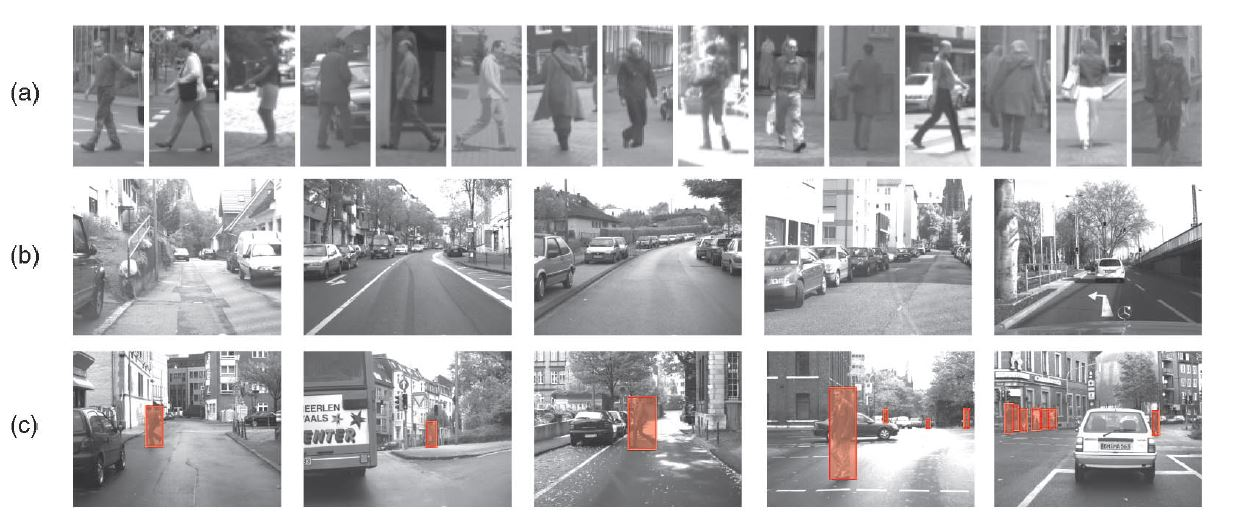
\includegraphics[width=7in]{fig1.JPG}
\caption{Overview of the Daimler pedestrian detection benchmark data set: (a) Pedestrian training samples, (b) nonpedestrian training images, (c) test
images with annotations.}
\end{figure*}

其次,基于组件的方法将行人外形分解为多个子部分.这些部分既受启发于语义学
(如头,躯干,腿等身体部分)\cite{bib2},\cite{bib45},\cite{bib48},
\cite{bib62},\cite{bib65},\cite{bib76}或是涉及到码本表示
\cite{bib1},\cite{bib39},\cite{bib40},\cite{bib61}.一般性的权衡被引入
到数量选择和个体部分选择中.
一方面,身体组件的空间尺度要尽可能小,以用于简便地
捕获关节活动.另一方面,身体组件必须要有充分大的空间尺度用以容纳可区分的
视觉结构,以实现可信检测.基于身体部分的方法需要整合局部部分响应
以得到最终决策的组合技术,最终决策受到各部分的空间关联限制.

采用分解为语义子区的方法训练出针对单一部分的可区分的基于特征的分类器
以及部分之间的几何关联模型.汇编基于部分的检测响应以得到最终分类结果
的技术包括组合分类器的训练\cite{bib2},\cite{bib48},\cite{bib62}和
给定观测图像特征条件下决定最佳对象构型的概率推断
\cite{bib45},\cite{bib65}
,\cite{bib76}.码书方法自底而上地将行人表示为局部码本特征的汇编,在图像
的突出点周围提取出来,并联合自上而下的验证\cite{bib39},\cite{bib40},
\cite{bib61}.

基于组件的方法与基于整体的分类相比具有显著优势.其并不受为充分覆盖可能外貌
集合的训练实例数量而带来的不利复杂度的影响.另外,由于场景重叠或是对象
间重叠所带来的丢失部分的期望值更容易得到处理,尤其是在显式对象间重叠
推理被联合到模型中时
\cite{bib39},\cite{bib40},\cite{bib61},\cite{bib76}.
但是,这些优势是以更高复杂度的模型生成(训练)和应用(测试)为代价的.由于
各组件检测器需要特定的空间支持以保持鲁棒性,其对低分辨率图像的适用
性受到限制.
\subsection{跟踪}
在跟踪行人以推测轨线层面的信息方面工作量相当大.研究的一条分支将跟踪阐述为
基于几何学和动力学的检测的逐帧关联,而没有特别的行人外貌模型\cite{bib2}
,\cite{bib23}.其它方法利用行人外貌模型(2.2节)与几何学以及动力学
联合的方法\cite{bib4},\cite{bib26},\cite{bib32},\cite{bib39},
\cite{bib43},\cite{bib50},\cite{bib55},\cite{bib58},\cite{bib65},
\cite{bib70},\cite{bib76},\cite{bib77},\cite{bib80},\cite{bib82}.
一些方法还在贝叶斯框架下进一步整合了检测和跟踪,将外貌模型和观测密度,
动力学以及后验状态密度的概率推测等结合起来.这时,单一线索
\cite{bib4},\cite{bib26},\cite{bib55},\cite{bib70},\cite{bib76}和
多元线索\cite{bib32},\cite{bib43},\cite{bib50},\cite{bib58},
\cite{bib65}都得到应用.

多元线索的整合\cite{bib66}涉及到联合各线索分离模型得到联合观测密度.
后验状态密度的推测通常被阐述为递归滤镜程序\cite{bib3}.粒子滤镜
\cite{bib30}由于其采用加权随机样本集合紧密拟合复杂现实世界多模型后
验密度的能力而得到广泛应用.和行人跟踪尤为相关的扩展涉及到离散/连续
状态空间的混合\cite{bib26},\cite{bib50}以及高效采样策略\cite{bib13},
\cite{bib32},\cite{bib36},\cite{bib44}.

现实世界行人跟踪的一个重要问题是如何处理图像中的多个目标.由此提出了
两种关于跟踪多对象的基本策略.首先,理论上最佳方法是通过并行推测构建一个
涉及到目标数量及其构型的联合状态空间.这会带来状态空间的明显增长和
变量维数扩张的问题.减少计算复杂度的解决方案引入了基于网格或是预
计算可信度\cite{bib32},\cite{bib69}和诸如Metropolis-Hastings采样
\cite{bib36}的精细重采样技术,分区采样\cite{bib44},或是退火粒子
滤镜\cite{bib13}.其次,一些方法对单一跟踪器限制对象数量
并采用多个跟踪器实例
\cite{bib31},\cite{bib35},\cite{bib50},\cite{bib52}.
虽然这种技术简化了状态空间表示,但需要初始化单一跟踪方法和分离邻接跟踪
的规则.典型做法是采用独立检测器程序来初始化一个新建跟踪.

结合独立检测器来得到建议密度趋向于通过引导对候选图像区域进行粒子重采样
来增加鲁棒性.多跟踪器实例之间的竞争机制通过启发式算法形成
\cite{bib35},\cite{bib50}.与联合状态空间方法相比,跟踪质量直接依赖
于用于初始化的联合对象检测器的性能.
\begin{figure*}[!t]
\centering
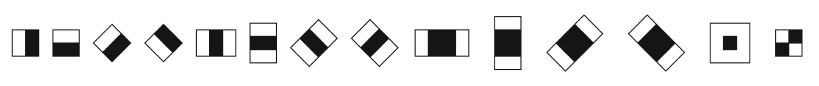
\includegraphics[width=5in]{fig2.JPG}
\caption{Overview of the employed set of Haar wavelets. Black and white areas denote negative and positive weights, respectively.}
\end{figure*}
\section{基准测试数据集}
Fig.~1展示了这项工作中采用的Daimler公司的行人检测基准测试数据集的摘录.
数据集统计在Table~1中.训练图像在不同的白天时间和地点进行记录,除了行人
都是保持直立姿势完全可见外,没有明亮度,行人姿势,或是衣着的限制.作为训练
实例的行人样本(阳性)有15,660个.这些样本通过从视频图像中人工提取出3,915
个矩形位置标签获取.每一个标签采用镜像或是在水平和垂直方向随机平移边界
框少量像素的方法创建4个行人样本,以考察应用系统的定位错误.附加的抖动样本
先前被证明能大幅提升性能\cite{bib14}.行人标签的最小高度是72像素,这样
一来鉴于所考察的系统的不同训练样本分辨率不会引入尺度放大.此外,我们提供
了6,744张不包含任何行人的图像,从这些图像中所有考察的方法将提取阴性训练
样本.

我们采用的测试数据集包括由21,790张图像($640\times480$像素)的独立图像序列,
连同56,492个人工标签,包括259个完全可视行人的轨迹,这些数据从运动车辆上
采集,耗时27分钟行驶于城市交通中.与其它现存的基准测试数据集(Table~1)
相比,以上数据的大小和复杂度使得我们能够下有
意义的结论,而没有可感知的过拟合效果.数据集总大小大概在8.5~GB左右.
\footnote{The data set is made freely available to academic and nonacademic
entities for research purposes. See \url{http://www.science.uva.nl/research/
isla/downloads/pedestrians/index.html} or contact the second author.}
\section{选择的行人检测方法}

我们选择了在特征(自适应,非自适应)和分类架构等方面采用不同
方法的多元集合用于评估(第5节):基于Haar小波的级联器\cite{bib74},
采用LRF特征的神经网络\cite{bib75},以及方向梯度直方图和线性SVM的结合
\cite{bib11}.除了这些滑窗类方法外,我们考察利用由粗到精形状匹配
和基于纹理的分类的系统,即\cite{bib23}的单眼视觉变体.时域整合通过采用2D边界
框跟踪器耦合.

我们承认,除了已选方案外,在单眼视觉行人检测领域还存在许多其它有趣的
研究支线(第2节).我们鼓励其他作者采用我们建议的数据集和基准测试
评估标准来报告性能.这里,我们聚焦于应用最广泛的方法.\footnote{
Total processing time for training, testing, and evaluation was several
months of CPU time on a 2.66 GHz Intel processor, using implementations
in C/C++.}

我们的实验配置设置底层系统参数(例如特征层和训练步骤)为原始出版物
\cite{bib11},\cite{bib23},\cite{bib49},\cite{bib74},\cite{bib75}
中报告的最佳参数.我们采用了两种不同的训练样本分辨率用于比较.我们以32像素(
小尺寸)和72像素(中尺寸)的实际行人高度考察训练样本.另外,我们添加了
一个固定的边界框像素.下文介绍具体细节.
\subsection{基于Haar小波的级联器}
基于Haar小波的级联器框架\cite{bib74}提供了一个高效滑窗方法扩展,引入了
复杂度递增检测层的退化决策树.每一层使用一个非自适应Haar小波特征集合
\cite{bib48},\cite{bib53}.我们在不同的尺寸和场景条件下采用Haar小波特征,
由水平方向和垂直方向特征,以及相应的倾斜的特征,连同点检测器,如Fig.~2所示.
小尺寸训练集合的样本分辨率为$18\times36$像素连同一个围绕行人的2像素的
边框.除了要求特征完全展现在训练样本中之外,没有对小波尺寸和场景加以任何限制.
可能的特征总数为154,190.中尺度训练集合包含$40\times80$像素以及一个围绕行人
的4像素边框的训练集合,可能的特征数超过350万个.因此,为了训练的可行性我们必须
对特征加以限制:我们要求空域重叠75\%的各特征具有24像素的最小区域,2像素的步长
,这样一来可能特征总数降为134,621个.在每一个级联层,AdaBoost算法\cite{bib18}
被用于构建一个基于已选特征加权线性组合的分类器,使得包含行人类和非行人类样本的
训练集合具有最低错误率.

我们考察在$N_l$层后的性能并发现在各种训练分辨率下当$N_l=15$时性能达到
饱和.每个级联层在包含新的初始的15,660个行人训练样本数据集和包含15,660个非行人
新样本下训练,非行人类的样本通过在给定非行人类集合图像下直到前级一层误判
为阳性的样本构建.第一层的阴性样本进行随机采样.每一层的性能准则
被设置为在99.5\%的检测率下50\%的阳性误判率.进一步增加级联层能减少训练错误,
但是针对测试集合的性能达到饱和.整个15层级联器在低(中)分辨率条件下由
AdaBoost算法选择的特征数为4,070(3751),从第一层的15(14)个特征递增到最后一层
的727(674)个特征.实验在用Intel OpenCV运算库\cite{bib29}提供的实现进行.

\begin{figure*}[!t]
\centering
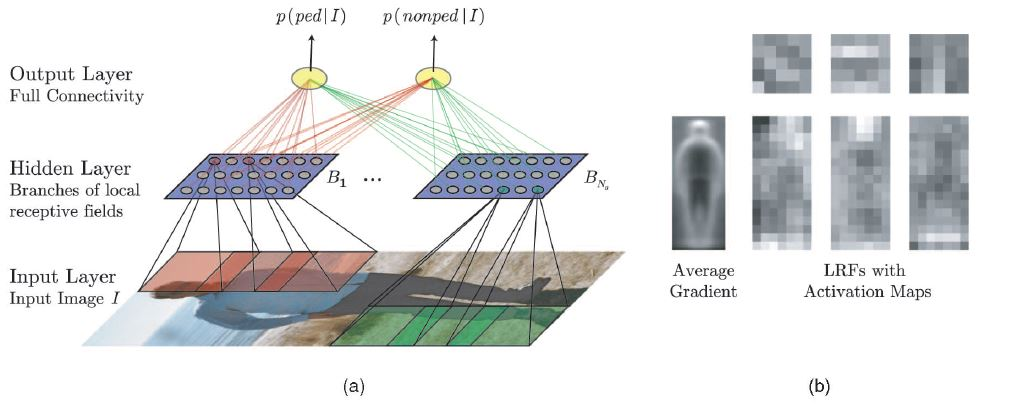
\includegraphics[width=7in]{fig3.JPG}
\caption{(a) Overview of NN/LRF architecture. (b) Average gradient image along with three exemplary $5\times5$-pixel local receptive field features (hidden
layer weights) and their activation maps (output layer weights) for the “pedestrian” output neuron, highlighting regions, where corresponding LRFs
are most discriminative for the pedestrian class.}
\end{figure*}
\subsection{采用局部感知域特征的神经网络(NN/LRF)}
适应性局部感知域(LRF)\cite{bib19}在行人检测领域被证明是一个有力特征,与一个
多层前馈神经网络架构结合(NN/LRF)\cite{bib75}.虽然LRF特征和非线性支持
向量机结合的分类(SVM/LRF)被证明具有稍好的性能\cite{bib49},我们仍选择
NN/LRF,因为由于超出内存限制,在我们的大数据集上训练SVM/LRF分类器是不可行的.

与隐藏层与输入层完全连接的多层感知器相比,NN/LRF引入了$N_B$个$B_i$分支的
概念($i=1,...,N_B$),每一条分支中的神经元值感知输入层的有限的局部区域,
即其感知域.如Fig.~3所示.因为突触加权(synaptical weights)在同一分支的
神经元之间共享,每一条分支可被视为一个输入模式上的空域特征检测器,待定
参数个数在训练期间减少,缓解对过拟合的敏感性.

\begin{figure*}[!t]
\centering
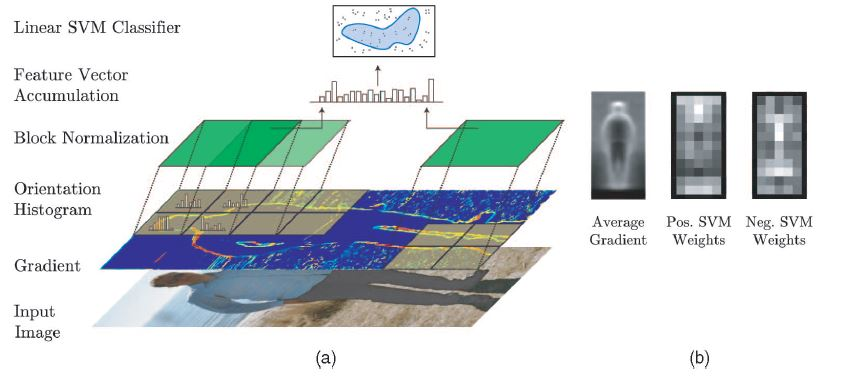
\includegraphics[width=7in]{fig4.JPG}
\caption{(a) Overview of HOG/linSVM architecture. Cells on a spatial grid are shown in yellow, whereas overlapping normalization blocks are shown in
green. (b) Average gradient image along with visualization of positive and negative SVM weights, which highlight the most discriminative regions for
both the pedestrian and nonpedestrian classes.}
\end{figure*}
我们采用一个$N_B=16$个$B_i$分支组成的NN/LRF.对于分辨率为$18\times36$
并带有一个2像素边框的小尺寸训练样本,采用$5\times5$像素的感知域,按照
2像素步长在训练图像上平移.$10\times10$像素的感知域按照5像素步长在
$40\times80$像素带有4像素边框的中尺寸训练样本上平移.

输出层由两个神经元组成,分别代表行人类和非行人类的后验概率估计.初始训练
数据由给定的15,660个行人样本以及15,560个从阴性图像中随机选择的样本.
我们进一步采用自展策略(bootstrapping strategy),在不包含行人的图像上
平移NN/LRF分类器,在每次迭代中收集15,660个误判为阳性的样本扩展阴性训
练集合.最后用扩展阴性训练数据重训练分类器.自展策略应用到测试性能饱和
为止.自展数据集合的更高的复杂度可以通过在每次迭代中结合附加的8个分支
来获得.

\begin{figure*}[!t]
\centering
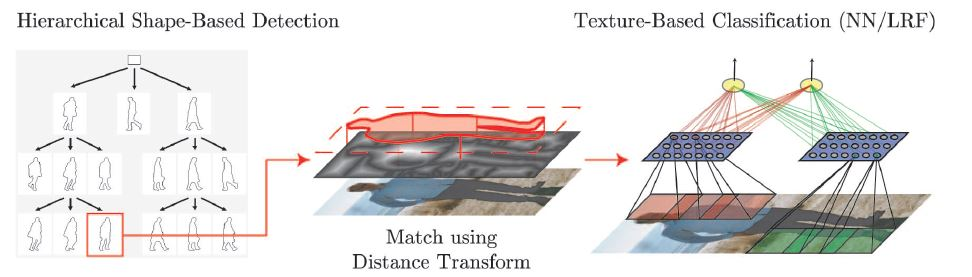
\includegraphics[width=7in]{fig5.JPG}
\caption{Overview of combined shape-based detection and texture-based classification.}
\end{figure*}

\subsection{方向梯度直方图特征和线性SVM的组合(HOG/linSVM)}
我们采用Dalal和Triggs的方法\cite{bib11}来构建局部形状和外貌模型,
如Fig.~4所示的标准化的方向梯度密度直方图(HOG).局部梯度根据其方向
分箱(binning),在包含重叠块对比归一化(blockwise contrast normalization)的空
域单元网格内根据其幅度加权.在每一个重叠块内,通过从空域单元对直方图
进行采样来提取特征向量.特征向量经过串联生成最终特征向量,然后递交
给采用线性支持向量机的分类器(linSVM).


系统参数的选择基于Dalal和Triggs的建议\cite{bib11}.与基于小波的Haar
级联器和NN/LRF相比,我们采用更大的边界来确保对梯度计算鲁棒性充足的空
域支持,并在行人边界上进行分箱(binning).这样,小尺寸训练样本采用
$22\times44$像素以及6像素边界的分辨率,中尺寸训练样本采用$48\times96$
像素以及12像素边界的分辨率.

我们采用了细尺度梯度((-1,0,1)无平滑化掩码),细方向分箱(9箱),粗空域分
箱(对$4\times4$的小尺寸和$8\times8$的中尺寸训练都采用$2\times2$块)
,以及重叠块对比归一化($L_2-norm$).描述符步长(descriptor stride)设定
为半块宽,以产生50\%的重叠.这相当于小尺寸4像素,相当于中尺寸8像素.

与NN/LRF的训练类似,初始的15,560个阴性样本从阴性图像中随机采样.我们在
每一次迭代中采用扩展训练集合(15,660个附加误判为阳性的样本)的自展技术直到性能
饱和.与NN/LRF分类器相反,线性SVM的复杂度在训练中通过在训练集合复杂
度增加的同时增加支持向量的数量来自动调整.实验在Dalal和Triggs提供的实
现\cite{bib11}下进行.

\subsection{联合形状-纹理行人检测}
我们考察了一个单眼视觉版本的实时保护装置系统\cite{bib23},将
基于形状的行人检测和基于纹理的行人分类级联.基于形状的检测器通过
由粗到精地用基于标本的形状层次(shape hierarchy)匹配待处理的图像
数据.形状层次用自动化的方法从手工注释的形状标签中离线构造,从训练
集合中的3,915个行人实例中提取.在线匹配引入了遍历形状层次中形状
模版和图像子窗口的Chamfer距离的精细鲁棒测量的方法.形状和图像之间
的相似度高于用户设定的门限值的图像区域被视为有效检测.每一层次的
距离门限值单独设定.附加的参数管理底层距离映射的边缘密度.所有参数
都采用序列ROC优化技术\cite{bib23}进行最优化.

形状匹配步骤的检测结果递交给基于纹理的模式分类器验证.这里,我们采用
在局部适应性感知域特征上操作的多层前馈神经网络(NN/LRF),使用
4.2节中给出的针对小尺寸训练集合的参数.如Fig.~5所示,初始的NN/LRF分
类器的阴性训练样本通过在给定的阴性训练图像集合上收集基于形状的检测
模块(使用宽松门限值)的误判为阳性的样本来提取.最后,对NN/LRF采用自展
技术.


\subsection{时域整合-跟踪}
检测结果的时域整合能克服检测缺陷,抑制寄生误判错误,并提供更高层次的
待检测对象的时域轨线信息.轨线层面的检测对于许多现实世界的关注焦点
或是风险评估策略来说是基础性的,如基于车辆的碰撞缓冲
系统或是视觉监督场景.在这项研究中,我们采用了基本的2D边界框跟踪器
连同一个包括边界框位置$(x,y)$和大小$(w,h)$的对象状态模型.对象状态
参数用$\alpha-\beta$跟踪器估计,包括经典Hungarian方法来进行数据分配
\cite{bib37}.当一个新对象连续出现在$m$帧中并且没有能够拟合的
现存跟踪器时,一个新建跟踪器开始运行.当与现存跟踪器相应的对象在$n$个
连续帧中都没被检测到时,相应的跟踪器停止运行.我们承认有更好的跟踪器
,如2.3节所示,其性能评估留待后人研究.我们采用的跟踪器的普遍性
和简洁性使得其具有允许直接整合进其它待考察的检测方法的优势.
\begin{figure*}[!b]
\centering
\large{\textbf{TABLE~2\\
Overview of Sliding Window Parameter Sets $S_i$ for Generic Evaluation
}}
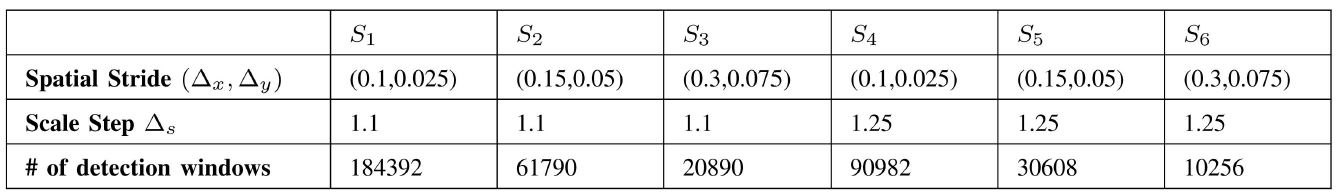
\includegraphics[width=7in]{table2.JPG}
\end{figure*}
\section{实验}
\subsection{方法学}
行人检测系统的性能评估基于采用建议的由21,790幅单眼视觉图像组成的
基准测试序列,将系统输出(报警)和人工标记的行人位置边界框所给出的实
际情况进行对比.我们对一般行人检测场景和接近于实时的车载行人检测场景
加以区分.前者在现实中存在很多可能的应用,从监控系统到机器人.后者针对
智能汽车\cite{bib20},\cite{bib23}中的碰撞缓冲/避免应用.两个场景在感兴趣
区域的定义以及匹配标准上有所差异.另外,车载场景对平均处理时间有所要求.

在两种场景中,我们考察多对多数据对应,即当在定位容差内至少有一个报警时事件
得到匹配.例如,系统并不要求检测出行人群体中的每一个行人个体.多元检测器在
近乎相同的地点和尺寸下的响应在所有方法中都需要进行编址,即通过应用基于
信赖度的非最大值抑制算法采用成对盒覆盖范围来检测边界
盒:两个系统报警$a_i$和$a_j$的覆盖范围
\[\Gamma(a_i,a_j)=\frac{A(a_i\cap{}a_j)}{A(a_i\cup{}a_j)}\]
即交集和并集的比率,如果高于$\theta_n$(我们在评估中设定为$\theta_n=0.5$),
将提交给非最大值抑制算法.具有最低信赖度的检测被丢弃,信赖度通过对检测器评估
得到,即:级联器(最后一层),NN/LRF和SVM的决策值.一种替代法采用基于核函数的投票
算法来决策检测出的边界盒的位置和大小\cite{bib10}.

性能评估同时在帧层面和轨迹层面进行.帧层面的性能通过在敏感度,精确度和
每帧阳性误判率等方面评估.敏感度和检测出的真解所占百
分比相关,精确度和正确系统解所占百分比相关.我们用
ROC曲线将帧层面的性能可视化,基于相应的匹配标准描述敏感度和每帧阳性误判率之间的
权衡.NN/LRF和HOG/linSVM技术的ROC曲线通过变化相应的检测器输
出门限来生成.至于基于小波的级联器和级联的形状-纹理行人检测系统,存在
多元门限(每一个级联模块都有一个)可同时变化来决定ROC性能.每一个多元
门限集合对应ROC空间中的一点,最终ROC曲线通过计算点云中的Pareto最佳前沿
(frontier)得到\cite{bib23}.

在时域整合(跟踪)合并后,轨线层面的性能通过匹配的可靠轨线(敏感度)
的百分比,正确系统轨线的百分比(精确度),以及每分钟的错误轨线来衡
量.我们对两种类型的轨线加以区分\cite{bib23}:至少有一个或
50\%事件得到匹配的"class-B"和"class-A"轨线."class-B"轨线包括
"class-A"轨线,但后者要求更强的应用性能.我们还进一步量化了合并跟踪
元件带来的帧层面上的阳性误判率的减少.
\subsection{一般行人检测}
在一般行人检测中,没有应用任何附加(3D)场景知识和限制.我们仅仅
把行人检测视为单一的2D问题,至少72像素高度的完全可视的真实行人
(Table~1)按要求标记,对应于现实世界中的1.5米高的行人位于25米
之外的摄像机.更小的或是部分不可见的行人和脚踏自行车者和机车驾驶
人对于无针对正确/错误/丢失检测的奖励/惩罚的系统是可选的.在我们
的实验中,我们单独地考察训练数据分辨率(第4节),检测器网格大小
,以及通过自展或级联来增加更多的阴性训练样本的效果.

联合形状-纹理检测器(4.4节)在这里被忽略因为基于
形状的检测元件提供了对可能行人位置的快速定位,之所以被采用主要
是由于其处理速度,而处理速度在这个测试场景中并不被考虑.而我们
单独地评估了NN/LRF分类器,因为它是联合形状-纹理检测系统
的第二个模块(也是更重要的模块).

这样我们总共有三种方法:基于Haar小波的级联器(4.1节),
NN/LRF(4.2节)以及HOG/linSVM(4.3节)等采用多量程
滑窗技术的方法.用$s$表示当前尺寸,检测窗口同时以$\Delta_s$的
步长因子和基础检测器窗口大小$W_x$和$W_y$的$s\Delta_x$和$s\Delta_y$分之一的大小
在$x$和$y$方向移动.最小
尺寸$s_{min}$对应于72像素的检测器窗口高度,最大尺寸$s_{max}$
根据检测器窗口能够适应图像来选择.这样一来,所有系统的检测器网
格是相同的.定义了空域步进(检测器网格分辨率)和尺寸的一些检测器
参数设置$S_i=(\Delta^i_x,\Delta^i_y,\Delta^i_s)$在所有方法中
都被考察,如Table~2所示.2D匹配标准基于系统报警$a_i$和实际事件
$e_j$之间的边界盒覆盖率,当$\Gamma(a_i,e_j)>\theta_m$时视为
正确检测($\theta_m=0.25$).结果如Figs.6,7,8所示.
\begin{figure*}[!t]
\centering
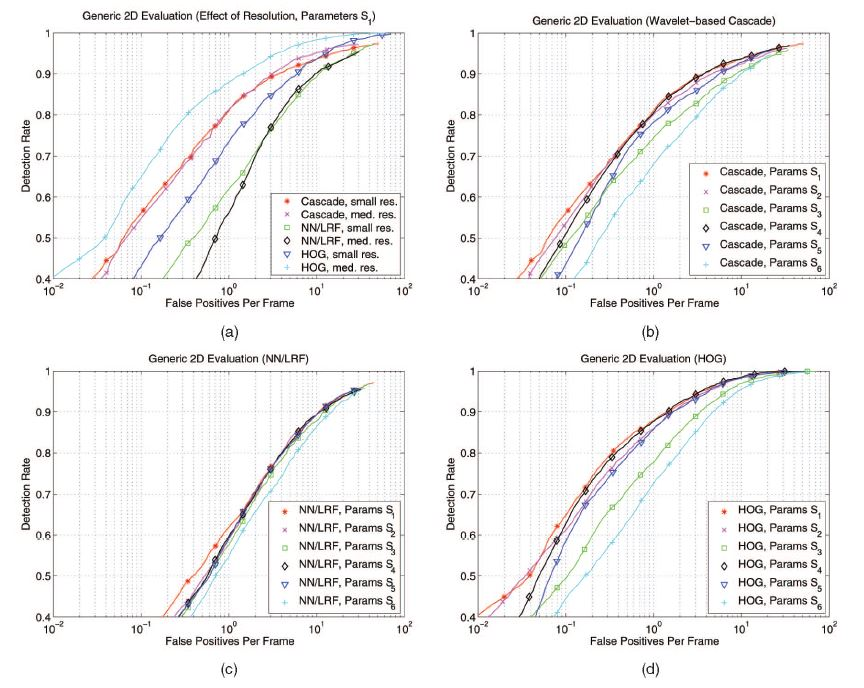
\includegraphics[width=6in]{fig6.JPG}
\caption{Evaluation of generic pedestrian detection. (a) Effect of different training resolutions. (b)-(d) Effect of varying detector grid for (b) waveletbased
cascade, (c) NN/LRF (1 bootstrapping iteration), and (d) HOG/linSVM (1 bootstrapping iteration).}
\end{figure*}

\begin{figure*}[!b]
\centering
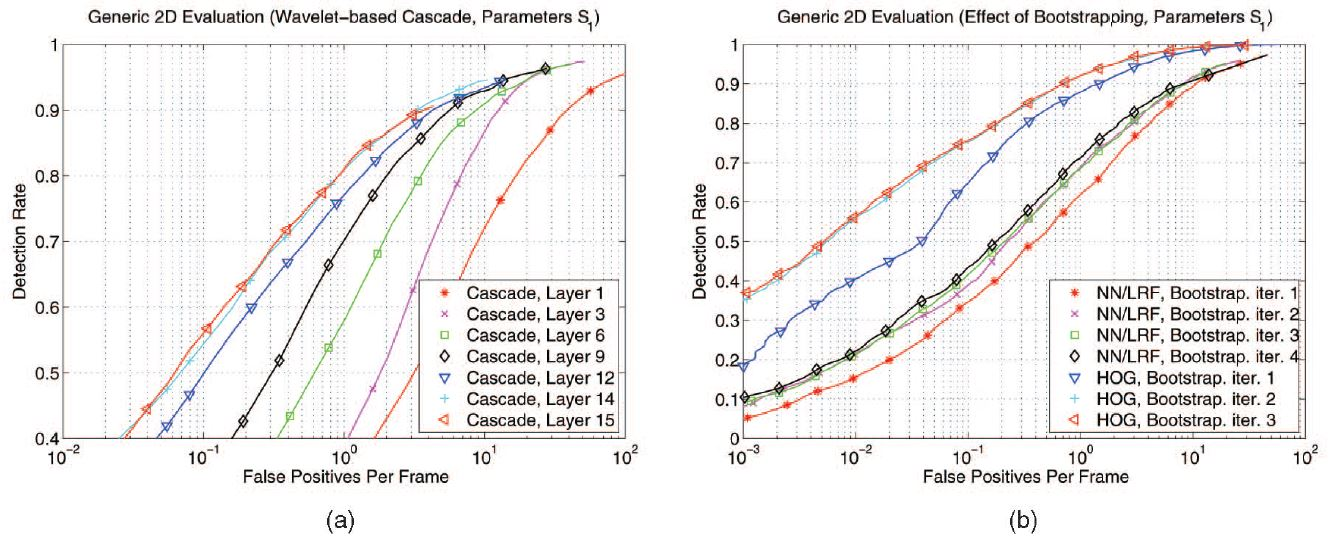
\includegraphics[width=5in]{fig7.JPG}
\caption{Evaluation of generic pedestrian detection. (a) Performance of individual cascade layers. (b) Effect of bootstrapping on NN/LRF and
HOG/linSVM.}
\end{figure*}
\begin{figure*}[!b]
\centering
\large{\textbf{TABLE~3\\
System Performance After Tracking F/A/B Denote Frame and Trajectory-Level Performance
}}
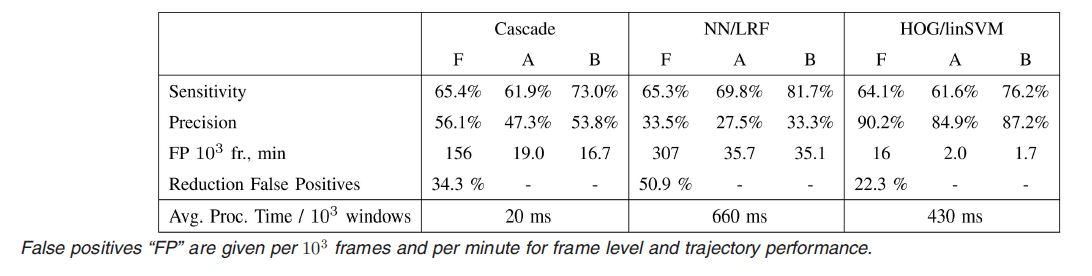
\includegraphics[width=7in]{table3.JPG}
\end{figure*}
Fig.~6a展示了采用$S_1$检测器参数时不同分辨率训练样本的效果.基于小波的
级联器和NN/LRF检测器在小分辨率和中分辨率之间的性能差异稍小,HOG/linSVM
在小尺寸图像场景下性能明显变差.造成这种情况的原因可能是小尺寸图像减少了
对直方图的空域支持.因此,进一步的实验只包括对各系统来说的最佳分辨率:基于小波
的级联器和NN/LRF检测器用小分辨率,HOG/linSVM方法采用中尺寸.

Figs.~6b,6c,6d展现了每一个检测器的定位容差(localization tolerance),即
对检测器网格颗粒度(granularity)的敏感性.我们从中观察到两点:首先,所有的
检测器在检测网格采用最佳颗粒度(参数$S_1$)时表现最佳.其次,各方法的定位
容差变化明显.NN/LRF在所有考虑的参数集合下性能几乎相同,最佳参数($S_1$)
和最差参数($S_6$)相比,在检测率不变的条件下每帧误判为阳性的数量减少了大
概1.5个因子.基于小波的级联器和HOG/linSVM方法对于检测网络分辨率表现出了
更强的敏感性,(最佳参数与最差参数)相比在误判为阳性方面大概分别减少了
3和5.5个因子.我们将这种现象归之于NN/LRF采用相对来说最大的特征(在
$18\times36$像素的样本上具有$5\times5$像素的感知域,4.2节),而
HOG/linSVM方法对$48\times96$像素的样本采用了$8\times8$像素的单元
(4.2节).如4.1节所示,基于小波的级联器采用了不同尺寸的特征.

\begin{figure}[!t]
\centering
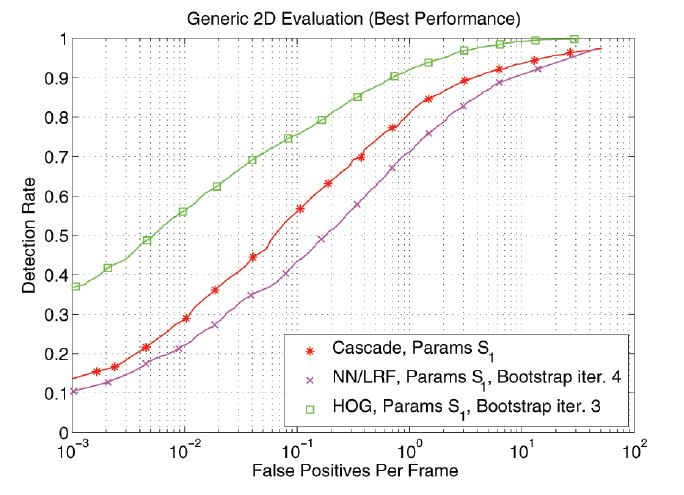
\includegraphics[width=3in]{fig8.JPG}
\caption{Evaluation of generic pedestrian detection: best performance of
each approach.}
\end{figure}
\begin{figure*}[!t]
\centering
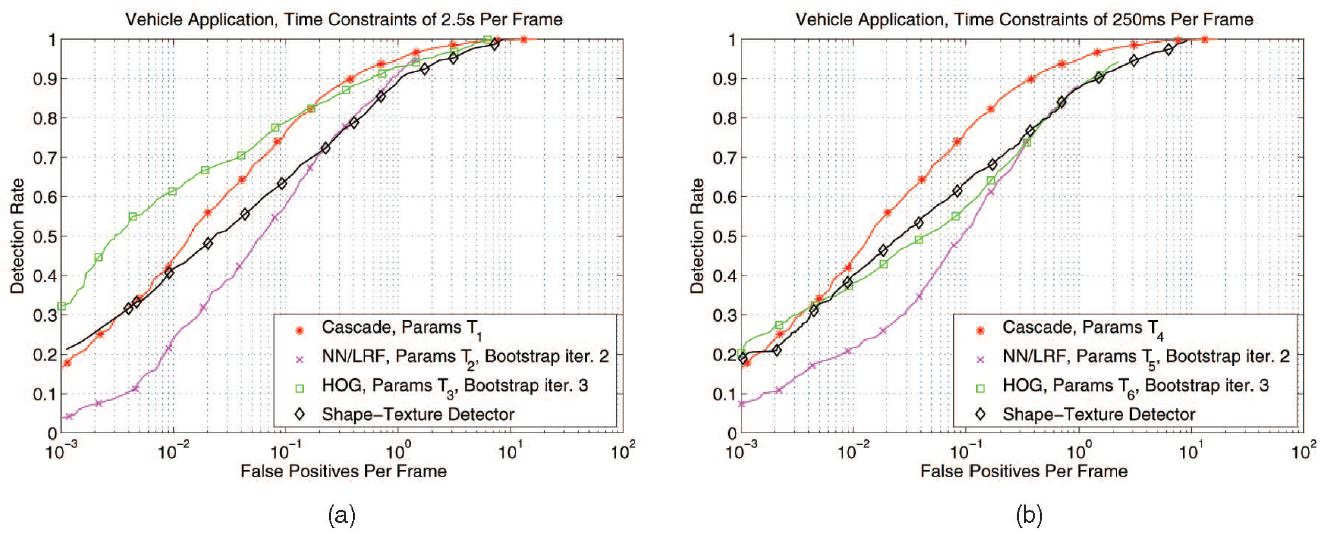
\includegraphics[width=7in]{fig9.JPG}
\caption{Results of onboard vehicle application using time constraints of (a) 2.5 s/frame and (b) 250 ms/frame.
}
\end{figure*}

在接下来的实验中,我们将检测器参数限制为相对各项技术来说的最佳设置
$S_1$.现在我们来评估附加阴性样本到训练集合的效果,对NN/LRF和
HOG/linSVM附加自展迭代,并展现基于小波的级联器的单层性能,每一层都
在不同的并且难度递增的阴性样本上训练.如Figs.~7a,7b所示.所有的检测器
都表现出性能增加,但分别在15层后(基于小波的级联器),3次迭代后(HOG/linSVM)
以及4次迭代后(NN/LRF)达到饱和.由于分类器在难度增加的训练集合下变得更加
复杂(NN/LRF的复杂度增加是按照设计的自展策略进行的,4.2节),
基于小波的级联器和NN/LRF检测器的性能提升是以计算消耗增加为代价的.
然而,对于HOG/linSVM检测器来说,评估中对于单个检测窗口的处理时间是
不变的.对于一个线性SVM,处理时间和支持向量组\cite{bib78}
的实际数量是独立的,随着自展迭代增加而增加.Fig.~8显示在测试数据集
上的每一个系统的最佳性能.HOG/linSVM方法明显胜过基于小波的级联器和
NN/LRF.在70\%的检测率下,HOG/linSVM检测器每帧误判为阳性的指数为0.045
,相比于基于小波的级联器为0.38,NN/LRF为0.86,分别减少了8个因子和19个
因子.

接下来,时域整合采用2D边界盒跟踪器(4.5节)
被合并到所有方法中,使用$m=2$和$n=2$的参数.跟踪器的输入是系统
检测以及通过对应的ROC曲线选择的系统参数,如Fig.~8所示,在60\%
敏感度的常数参考点上进行.结果如Table~3所示.我们观察到Fig.~8
所示的性能差异在合并跟踪后仍然存在.与基于小波的及联合和NN/LRF
检测器相比,HOG/linSVM方法在相同的敏感度级别下明显具有更高的
精确度.
\subsection{车载应用场景}
\begin{figure*}[!b]
\centering
\large{\textbf{TABLE~4\\
Overview of Sliding Window Parameter Sets $T_i$ for Onboard Vehicle Evaluation
}}
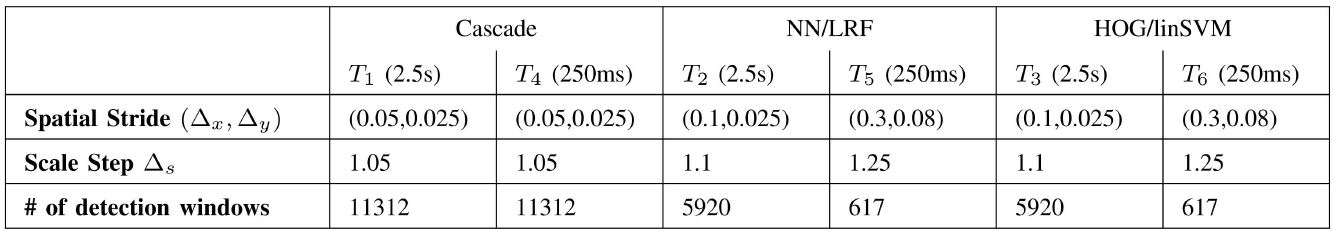
\includegraphics[width=7in]{table4.JPG}
\end{figure*}
在行驶车辆上的(接近于)实时的行人检测方面,应用限定要求在3D条件.
具体来说,传感器覆盖区域的定义和车辆相关,$10-25$米的纵向宽度以及
$\pm4$米的横向宽度.给定系统警报$a_i$和真实事件$e_j$,我们采用
一个3D最大位置偏差来对匹配进行计数,2D真实事件和2D检测采用
已知的摄像机几何学知识和行人都站在地面上(地平面限制)的假设
投影为3D图像.由于这种地平面限制只在完全可见行人的条件下可行,
部分可见的可视行人并不会投影为3D,而是在2D条件下同一个
$\theta_m=0.25$的边界盒覆盖率来进行匹配,如5.2节所示.
只考察和要求在传感器覆盖区域内的完全可视的真实行人(Table~1).
部分可见的行人和处于传感器覆盖区域之外的行人检测被视为可选的
(即,检测不进行奖惩).

横向(X)和纵向(Z)的定位容差被定义为占车辆的距离百分比.
这里,我们考察$X=10\%$和$Z=30\%$的容差,在将真实行人和检测
(单眼视觉)投影为3D时,纵向容差稍大是为了应对不平整的路面
以及车辆纵倾,即,在20米的距离时,我们接受
横向$\pm2$米以及纵向$\pm6$米的定位误差.

所有的系统都通过将3D场景知识合并到检测程序中得到评估:我们
假设1.5-2.0米高度的行人站在地面上.违背此假设的初始对象假设
会被忽略.不平整的路面和车辆纵倾通过采用$\phi=\pm2$度的纵倾角
容限来放宽地平面限制来建模.

我们考察了每张图片$2.5$秒和$250$毫秒的平均处理时间限制
($\pm10\%$的容差).为了采用这些限制,我们选择保持基本系统参数,
例如,原始作者报告的特征层样本分辨率,见第4节.我们采用
检测网格的大小来代表处理速度.服从于处理时间限制的滑窗参数$T_i$
在Table~4中给定.检测网格在y方向要比x方向去毛化(grained)得更精细.
这造成了在y方向局部精确度要高一些,这通过了将检测投影到3D增加了
深度估计的鲁棒性.除了滑窗技术,联合形状纹理检测器采用了由粗到精的
层次形状匹配方案来从每张图像中生成数量不等的ROI,递交给后级的
NN/LRF分类器.因此,形状匹配模块的层次级别的门限对处理时间影响最大.
我们将时间限制整合进参数最优化\cite{bib23},对给定处理时间要求
的门限进行最优化.

性能评估在15层级联条件下进行,形状纹理检测器以及HOG/linSVM和NN/LRF
方法在每次自展后寻求在给定时间限制下性能和处理时间之间的最佳权衡.
与一般评估相比,由于对于更复杂的NN/LRF检测器的计算消耗为了满足
时间限制必须大幅度缩小检测网格的分辨率,NN/LRF分类器在第二次自展
迭代后性能达到饱和.至于基于小波的级联器,相同的参数设置$T_1$和$T_1$
在两种时间限定设置下被采用.这是由于即使在250毫秒每帧的时间限制
下由于每一个检测窗口可以迅速得到评估而造成了非常紧密的检测网格
分辨率.进一步的增加网格分辨率并不会产生任何性能改进.我们将其归之于
训练数据的预处理,使得局部误差鲁棒性按照平移训练标签数个像素来得到
显式建模,如第3节中所描述.结果在Figs.~9a,9b中给出.

在2.5秒每帧的时间限制下,所有检测器的相关性能曲线和一般评估条件下类似
,如Figs.8,9a所示.与单独采用NN/LRF相比,联合形状纹理检测器进一步改善了
性能,尤其是在低阳性误判率的条件下.进一步的限定250毫秒每帧的处理时间,
HOG/linSVM检测器的性能急剧下降,然而NN/LRF的性能只是稍微降低.这同样是
不同的定位容差的作用,如第5.2节评估所示.联合形状纹理检测器的性能
几乎不变.这说明形状检测模块强大的剪枝能力使得后级高计算消耗的纹理分类器
专注于处理可能的图像区域,这样便减小了计算消耗.在紧处理时间限定下,
得益于其高速处理速度,基于小波的级联器明显胜过我们考察的其它方法.
联合形状纹理检测器以明显的劣势性能其次.

\begin{figure*}[!t]
\centering
\large{\textbf{TABLE~5\\
System Performance After Tracking
}}
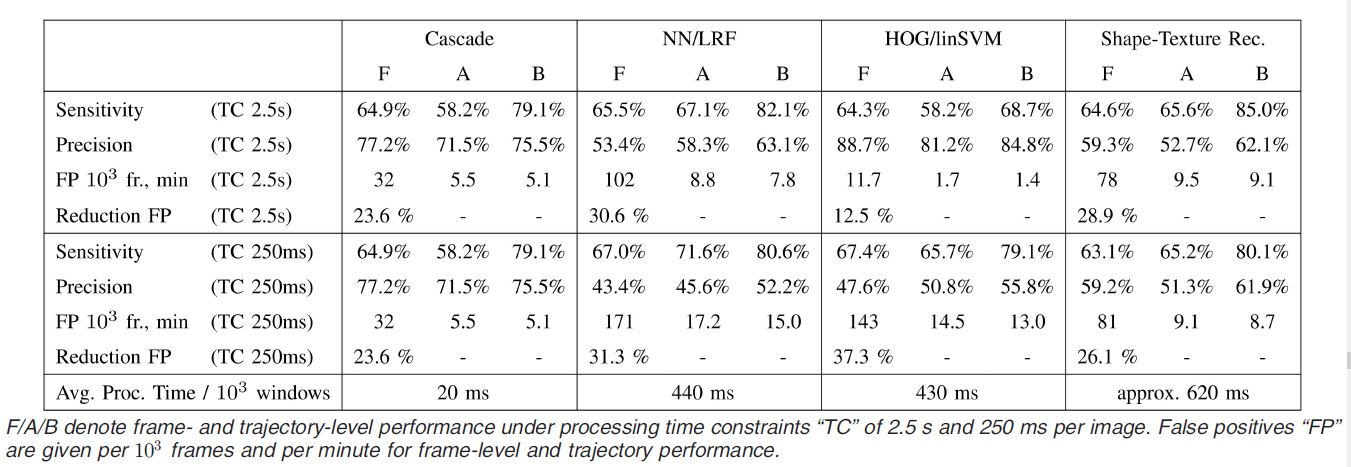
\includegraphics[width=7in]{table5.JPG}
\end{figure*}
在一般行人检测场景下(5.2节),合并了边界盒跟踪器.作为一般参考点,
我们再一次采用从Figs.~9a,9b所示的ROC曲线中获取的60\%这一敏感度.
结果在Table~5中给出.在两种时间限定设置下,Figs.9a,9b显示相关的各系统
性能排序并没有改变.然而,我们能够观测到跟踪器的良性效果的差异.除
HOG/linSVM之外的所有系统,跟踪器带来的良性效果在两种时间限制设定下
相似,大概在25-35\%之间,如Table~5所示.对于HOG/linSVM检测器在2.5秒每帧
的时间限定下,许多错误检测变得强时域相关并且不能被跟踪器消除.阳性误判率
值只减少了12.5\%.在250毫秒每帧的时间限定下跟踪器对HOG/linSVM的
效果更好,因为每幅图像有更少的检测窗口得到评估.为了达到60\%的
敏感度,需要一个更宽松的门限设置.结果引进了更多的误判,我们观测到
这些误判更弱的时域相关性;这些误判可以通过跟踪器抑制.

在2.66GHz的Intel处理器上采用C/C++实现的条件下,每$10^3$次检测窗口
的平均处理时间在Table~5中给出.与其它技术相比,基于小波的级联器架构
在处理时间方面具有巨大优势,大概快20倍.注意到联合形状纹理检测器
具有最快每检测窗口处理速度.然而,由于通过由粗到精的形状匹配模块
得到的搜索空间的有效剪枝,每幅图像的检测窗口数量与滑窗技术相比
在保持相似性能级别的条件下大量减少.
\section{讨论}
我们得到一个关于某些待测方法的相关性能的微妙情况,这些待测方法依赖于
行人图像分辨率和用于探测的空域网格大小(作为处理速度的代表).在
低分辨率行人图像场景下(如$18\times36$像素),密集型Haar小波特征
最为可行.另一方面,HOG特征在中尺寸场景下表现最好($如48\times96$
像素).这些方法由于需要更大的空域支持而限制了在某些应用场景中的
使用,例如,采用5.3节中的摄像机设置,行人在车辆25米之外时在
图像中的高度小于72像素.我们期望用基于组件或是码书的方法
\cite{bib1},\cite{bib39},\cite{bib40},\cite{bib61}来作为那些
需要更高分辨率的行人图像的应用的选择.

\begin{figure*}[!t]
\centering
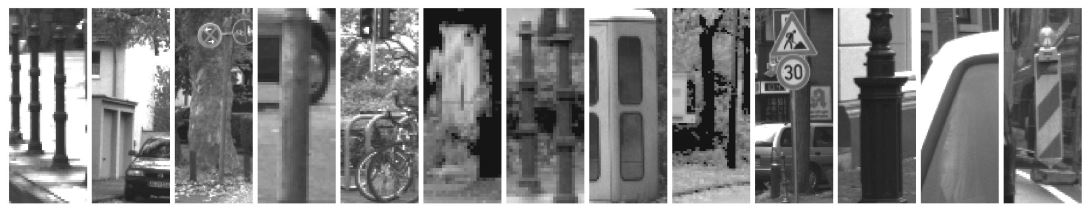
\includegraphics[width=7in]{fig10.JPG}
\caption{Typical false positives of all systems. Most errors occur in local regions with strong vertical structure.
}
\end{figure*}
从整个系统来说,实验结果表明基于HOG的线性SVM方法在中尺寸行人图像
分辨率和低处理速度场景下具有明显优势,并且基于小波的AdaBoost级联器
在低分辨率行人图像和(接近于)实时处理速度的场景下性能最好.理所当然,
跟踪器提升了所有考察的系统的性能,并且减少了系统之间性能差异.我们
注意到,虽然这项研究中接受测试的系统基于不同的特征,他们都会犯相似
的错误.对于所有系统来说,典型的误判发生在显示出强纵向结构的局部区域
,如Fig.~10所示.

通过比较在实际应用中的必要因素来部署本文获取的最佳性能是有意义的.
我们考察5.3节中描述的智能车辆应用.如果我们假设有一个采用单眼
视觉的辅助系统向驾驶员发出关于可能发生行人碰撞的语音警告,从轨迹
层面来讲超过80\%的正确检测率被视为足够敏感,也就是说,在城市交通
中10小时的驾驶内产生的错误警报不超过1次.在250毫秒每帧的条件下
(假设最优化对实时实现有用)各种系统的测试结果如Table~5显示,我们
注意到基于小波的级联器的最佳性能大概为每分钟6次错误轨线以及60\%
的检测率.或许有人会做出尚存在3个数量级的性能差距.这或许过于悲观
了,因为Table~5反映了在已定义的覆盖区域内的所有行人轨线的平均性能
(高达10-25米$\pm4$米的横向距离).实际中,碰撞相关的轨线趋于更长并且
个体检测在其更接近于车辆的情况下更容易.我们的初步调查显示在实际
轨线子集场景下检测性能能够提高1个数量级,然而还是与理想的性能存在
2个数量级的差异.

如何缩小性能差异呢?最有效的方法是结合一个预处理阶段来限制图像搜索
空间,如基于可选的线索:行为\cite{bib15},\cite{bib56},深度
\cite{bib7},\cite{bib23},\cite{bib81}.例如,\cite{bib23}报告通过
引入基于立体的障碍物检测能够带来1个数量级的性能增益(或许可以通过
结合背景减除[background sutraction]的监督设置来获取相似的性能增加).

剩下的性能增益(即上述智能车辆应用中的1个数量级的性能差异)或许需要
从分类方法的改善中获取.例如,在4.4节中描述的形状纹理技术,
层次化的形状匹配引入概率方法能够获取性能提升\cite{bib22}.
特殊形状已匹配模版可以进一步索引入一个分类器集合(专家),每一个
代表一个特别身体姿势.Gavrila和Munder\cite{bib23}报告显示这种
混合专家架构能够提升大约30\%的性能.级联器技术可以和更强大的特征
组合,例如,局部感知域(4.2节)或是梯度直方图(4.3节).
Zhu等人\cite{bib83}完成了采用HOG特征的级联检测器的初始工作
并且报告显示实时处理速度下与原始HOG/linSVM技术相近的性能级别
\cite{bib11}.

或许,数据集才是最关键的.最近的一项关于行人分类的研究\cite{bib49}
显示选择特征和模式分配器的最佳组合带来的效果不如优化训练集合明显,
虽然现有的基础训练集合已经包含了数以千计的样本\cite{bib49}.
\section{结论}
这篇文章从理论和实验的视角对最近在单眼行人检测领域的工作做出综述.
为了在一般和特殊之间权衡,我们考察了两种评估设定:一般设定(没有场景
和处理限制的条件下进行),以及运动车载场景的特殊应用.

实验结果显示出某些接受测试的方法的相关性能的微妙情况,这些方法
依赖于行人图像分辨率和用于探测的空域网格大小(作为处理速度的代表).
基于HOG的线性SVM方法在没有或是很小的处理时间限制条件下比其它方法
都表现得好(分别在没有时间限制和2.5秒每帧的时间限制条件下比其他方法
少了10-18和3-6个A类错误轨线因子).这说明基于局部边缘方向的特征表示
擅长于捕获行人对象类的复杂外貌.在加以更紧的处理速度限制后,基于小波
的Haar级联器方法表现最优(在250毫秒每帧的条件下比其它方法少了2-3
个A类错误轨线因子).

对于所有系统来说,通过结合时域整合或是基于场景知识限制搜索空间能够
提升性能.跟踪器元件趋于减少个方法之间的性能差异.从实际应用的角度
来说,错误轨线的数量过高(至少1个数量级),这说明在这项复杂但是重要
的问题上还需要很多未来的努力.
%Single Column Floating Figure
%\begin{figure*}[!t]
%\centering
%\includegraphics[width=5in]{myfigure.pdf}
%\caption{Simulation Results.}
%\label{fig_sim}
%\end{figure*}

%double column floating figure
%\begin{figure*}[!t]
%\centering
%\subfloat[Case I]{\includegraphics[width=2.5in]{box}%
%\label{fig_first_case}}
%\hfil
%\subfloat[Case II]{\includegraphics[width=2.5in]{box}%
%\label{fig_second_case}}
%\caption{Simulation results.}
%\label{fig_sim}
%\end{figure*}

%Floating Table
%\begin{table}[!t]
%\renewcommand{\arraystretch}{1.3}
%\caption{An Example of a Table}
%\label{table_example}
%\centering
%\begin{tabular}{|c||c|}
%\hline
%One & Two\\
%\hline
%Three & Four\\
%\hline
%\end{tabular}
%\end{table}


\section*{Acknowledgment}
The authors acknowledge the support of the Studienstiftung
des deutschen Volkes and Bundesministerium f\"ur Wirtschaft und
Technologie, BMWi in the context of the AKTIV-SFR
initiative. They furthermore thank Professor Dr. Christoph
Schn\"o rr (Image and Pattern Analysis Group, University of
Heidelberg, Germany), who provided helpful comments
and discussions.

% bibliography section
\begin{thebibliography}{99}
\bibitem{bib1}
S. Agarwal, A. Awan and D. Roth, "Learning to Detect Objects in Images via a Sparse, Part-Based Representation," IEEE Trans. Pattern Analysis and Machine Intelligence, vol. 26, no. 11, pp. 1475-1490, Nov. 2004. 
\bibitem{bib2}
I.P. Alonso et al. "Combination of Feature Extraction Methods for SVM Pedestrian Detection," IEEE Trans. Intelligent Transportation Systems, vol. 8, no. 2, pp. 292-307, June 2007. 
\bibitem{bib3}
S. Arulampalam, S. Maskell, N. Gordon and T. Clapp, "A Tutorial on Particle Filters for On-Line Non-Linear/Non-Gaussian Bayesian Tracking," IEEE Trans. Signal Processing, vol. 50, no. 2, pp. 174-188, Feb. 2002.
\bibitem{bib4}
A. Baumberg, "Hierarchical Shape Fitting Using an Iterated Linear Filter," Proc. British Machine Vision Conf., pp. 313-323, 1996. 
\bibitem{bib5}
M. Bergtholdt, D. Cremers and C. Schnö,rr, "Variational Segmentation with Shape Priors," Handbook of Math. Models in Computer Vision, N. Paragios, Y. Chen, and O. Faugeras, eds., Springer, 2005. 
\bibitem{bib6}
G. Borgefors, "Distance Transformations in Digital Images," Computer Vision, Graphics, and Image Processing, vol. 34, no. 3, pp. 344-371, 1986.
\bibitem{bib7}
A. Broggi, A. Fascioli, I. Fedriga, A. Tibaldi and M.D. Rose, "Stereo-Based Preprocessing for Human Shape Localization in Unstructured Environments," Proc. IEEE Intelligent Vehicles Symp., pp. 410-415, 2003. 
\bibitem{bib8}
T.F. Cootes, S. Marsland, C.J. Twining, K. Smith and C.J. Taylor, "Groupwise Diffeomorphic Non-Rigid Registration for Automatic Model Building," Proc. European Conf. Computer Vision, pp. 316-327, 2004. 
\bibitem{bib9}
T.F. Cootes and C.J. Taylor, "Statistical Models of Appearance for Computer Vision," technical report, Univ. of Manchester, 2004. 
\bibitem{bib10}
N. Dalal, "Finding People in Images and Videos," PhD thesis, Institut Nat',l Polytechnique de Gre noble, 2006. 
\bibitem{bib11}
N. Dalal and B. Triggs, "Histograms of Oriented Gradients for Human Detection," Proc. IEEE Int',l Conf. Computer Vision and Pattern Recognition, pp. 886-893, 2005. 
\bibitem{bib12}
N. Dalal, B. Triggs and C. Schmid, "Human Detection Using Oriented Histograms of Flow and Appearance," Proc. European Conf. Computer Vision, pp. 428-441, 2006. 
\bibitem{bib13}
J. Deutscher, A. Blake and I.D. Reid, "Articulated Body Motion Capture by Annealed Particle Filtering," Proc. IEEE Int',l Conf. Computer Vision and Pattern Recognition, pp. 126-133, 2000. 
\bibitem{bib14}
M. Enzweiler and D.M. Gavrila, "A Mixed Generative-Discriminative Framework for Pedestrian Classification," Proc. IEEE Int',l Conf. Computer Vision and Pattern Recognition, 2008. 
\bibitem{bib15}
M. Enzweiler, P. Kanter and D.M. Gavrila, "Monocular Pedestrian Recognition Using Motion Parallax," Proc. IEEE Intelligent Vehicles Symp., pp. 792-797, 2008. 
\bibitem{bib16}
A. Ess, B. Leibe and L. van Gool, "Depth and Appearance for Mobile Scene Analysis," Proc. Int',l Conf. Computer Vision, 2007. 
\bibitem{bib17}
L. Fan, K.-K. Sung and T.-K. Ng, "Pedestrian Registration in Static Images with Unconstrained Background," Pattern Recognition, vol. 36, pp. 1019-1029, 2003. 
\bibitem{bib18}
Y. Freund and R.E. Schapire, "A Decision-Theoretic Generalization of On-Line Learning and an Application to Boosting," Proc. European Conf. Computational Learning Theory, pp. 23-37, 1995. 
\bibitem{bib19}
K. Fukushima, S. Miyake and T. Ito, "Neocognitron: A Neural Network Model for a Mechanism of Visual Pattern Recognition," IEEE Trans. Systems, Man, and Cybernetics, vol. 13, pp. 826-834, 1983. 
\bibitem{bib20}
T. Gandhi and M.M. Trivedi, "Pedestrian Protection Systems: Issues, Survey, and Challenges," IEEE Trans. Intelligent Transportation Systems, vol. 8, no. 3, pp. 413-430, Sept. 2007. 
\bibitem{bib21}
D.M. Gavrila, "The Visual Analysis of Human Movement: A Survey," Computer Vision and Image Understanding, vol. 73, no. 1, pp. 82-98, 1999. 
\bibitem{bib22}
D.M. Gavrila, "A Bayesian Exemplar-Based Approach to Hierarchical Shape Matching," IEEE Trans. Pattern Analysis and Machine Intelligence, vol. 29, no. 8, pp. 1408-1421, Aug. 2007. 
\bibitem{bib23}
D.M. Gavrila and S. Munder, "Multi-Cue Pedestrian Detection and Tracking from a Moving Vehicle," Int',l J. Computer Vision, vol. 73, no. 1, pp. 41-59, 2007. 
\bibitem{bib24}
B.E. Goldstein, Sensation and Perception, sixth ed. Wadsworth, 2002. 
\bibitem{bib25}
T. Heap and D. Hogg, "Improving Specificity in PDMs Using a Hierarchical Approach," Proc. British Machine Vision Conf., pp. 80-89, 1997. 
\bibitem{bib26}
T. Heap and D. Hogg, "Wormholes in Shape Space: Tracking through Discontinuous Changes in Shape," Proc. Int',l Conf. Computer Vision, pp. 344-349, 1998. 
\bibitem{bib27}
B. Heisele and C. Wö,hler, "Motion-Based Recognition of Pedestrians," Proc. Int',l Conf. Pattern Recognition, pp. 1325-1330, 1998. 
\bibitem{bib28}
INRIA Person Dataset, http://pascal.inrialpes.fr/data/human/, 2007. 
\bibitem{bib29}
Intel OpenCV Library, http://www.intel.com/technology/ computing/opencv/, 2007. 
\bibitem{bib30}
M. Isard and A. Blake, "CONDENSATION\&mdash,Conditional Density Propagation for Visual Tracking," Int',l J. Computer Vision, vol. 29, no. 1, pp. 5-28, 1998. 
\bibitem{bib31}
M. Isard and A. Blake, "ICONDENSATION: Unifying Low-Level and High-Level Tracking in a Stochastic Framework," Proc. Int',l Conf. Computer Vision, pp. 893-908, 1998. 
\bibitem{bib32}
M. Isard and J. MacCormick, "BraMBLE: A Bayesian Multiple-Blob Tracker," Proc. Int',l Conf. Computer Vision, pp. 34-41, 2001. 
\bibitem{bib33}
A.K. Jain, R.P.W. Duin and J. Mao, "Statistical Pattern Recognition: A Review," IEEE Trans. Pattern Analysis and Machine Intelligence, vol. 22, no. 1, pp. 4-37, Jan. 2000. 
\bibitem{bib34}
M.J. Jones and T. Poggio, "Multidimensional Morphable Models," Proc. Int',l Conf. Computer Vision, pp. 683-688, 1998. 
\bibitem{bib35}
H. Kang and D. Kim, "Real-Time Multiple People Tracking Using Competitive Condensation," Pattern Recognition, vol. 38, no. 7, pp. 1045-1058, 2005. 
\bibitem{bib36}
Z. Khan, T. Balch and F. Dellaert, "MCMC-Based Particle Filtering for Tracking a Variable Number of Interacting Targets," IEEE Trans. Pattern Analysis and Machine Intelligence, vol. 27, no. 11, pp. 1805-1819, Nov. 2005. 
\bibitem{bib37}
H.W. Kuhn, "The Hungarian Method for the Assignment Problem," Naval Research Logistics Quarterly, vol. 2, pp. 83-97, 1955. 
\bibitem{bib38}
S. Lee, Y. Liu and R. Collins, "Shape Variation-Based Frieze Pattern for Robust Gait Recognition," Proc. IEEE Int',l Conf. Computer Vision and Pattern Recognition, 2007. 
\bibitem{bib39}
B. Leibe, N. Cornelis, K. Cornelis and L.V. Gool, "Dynamic 3D Scene Analysis from a Moving Vehicle," Proc. IEEE Int',l Conf. Computer Vision and Pattern Recognition, 2007. 
\bibitem{bib40}
B. Leibe, E. Seemann and B. Schiele, "Pedestrian Detection in Crowded Scenes," Proc. IEEE Int',l Conf. Computer Vision and Pattern Recognition, pp. 878-885, 2005. 
\bibitem{bib41}
R. Lienhart and J. Maydt, "An Extended Set of Haar-Like Features for Rapid Object Detection," Proc. Int',l Conf. Image Processing, pp. 900-903, 2002. 
\bibitem{bib42}
D.G. Lowe, "Distinctive Image Features from Scale Invariant Keypoints," Int',l J. Computer Vision, vol. 60, no. 2, pp. 91-110, 2004. 
\bibitem{bib43}
J. MacCormick and A. Blake, "Partitioned Sampling, Articulated Objects and Interface-Quality Hand Tracking," Proc. European Conf. Computer Vision, pp. 3-19, 2000. 
\bibitem{bib44}
J. MacCormick and A. Blake, "A Probabilistic Exclusion Principle for Tracking Multiple Objects," Int',l J. Computer Vision, vol. 39, no. 1, pp. 57-71, 2000. 
\bibitem{bib45}
K. Mikolajczyk, C. Schmid and A. Zisserman, "Human Detection Based on a Probabilistic Assembly of Robust Part Detectors," Proc. European Conf. Computer Vision, pp. 69-81, 2004. 
\bibitem{bib46}
MIT CBCL Pedestrian Database, http://cbcl.mit.edu/cbcl/ software-datasets/PedestrianData.html, 2008. 
\bibitem{bib47}
T.B. Moeslund and E. Granum, "A Survey of Advances in Vision-Based Human Motion Capture and Analysis," Computer Vision and Image Understanding, vol. 103, nos. 2/3, pp. 90-126, 2006. 
\bibitem{bib48}
A. Mohan, C. Papageorgiou and T. Poggio, "Example-Based Object Detection in Images by Components," IEEE Trans. Pattern Analysis and Machine Intelligence, vol. 23, no. 4, pp. 349-361, Apr. 2001. 
\bibitem{bib49}
S. Munder and D.M. Gavrila, "An Experimental Study on Pedestrian Classification," IEEE Trans. Pattern Analysis and Machine Intelligence, vol. 28, no. 11, pp. 1863-1868, Nov. 2006. 
\bibitem{bib50}
S. Munder, C. Schnö,rr and D.M. Gavrila, "Pedestrian Detection and Tracking Using a Mixture of View-Based Shape-Texture Models," IEEE Trans. Intelligent Transportation Systems, vol. 9, no. 2, pp. 333-343, June 2008. 
\bibitem{bib51}
C. Nakajima, M. Pontil, B. Heisele and T. Poggio, "Full-Body Recognition System," Pattern Recognition, vol. 36, pp. 1997-2006, 2003. 
\bibitem{bib52}
K. Okuma, A. Taleghani, N. de Freitas, J. Little and D. Lowe, "A Boosted Particle Filter: Multitarget Detection and Tracking," Proc. European Conf. Computer Vision, pp. 28-39, 2004.
\bibitem{bib53}
C. Papageorgiou and T. Poggio, "A Trainable System for Object Detection," Int',l J. Computer Vision, vol. 38, pp. 15-33, 2000.
\bibitem{bib54}
PETS Data sets, http://www.cvg.rdg.ac.uk/slides/pets.html, 2007. 
\bibitem{bib55}
V. Philomin, R. Duraiswami and L.S. Davis, "Quasi-Random Sampling for Condensation," Proc. European Conf. Computer Vision, pp. 134-149, 2000. 
\bibitem{bib56}
R. Polana and R. Nelson, "Low-Level Recognition of Human Motion," Proc. IEEE Workshop Motion of Non-Rigid and Articulated Objects, pp. 77-92, 1994. 
\bibitem{bib57}
R. Poppe, "Vision-Based Human Motion Analysis: An Overview," Computer Vision and Image Understanding, vol. 108, pp. 4-18, 2007. 
\bibitem{bib58}
D. Ramanan, A.D. Forsyth and A. Zisserman, "Strike a Pose: Tracking People by Finding Stylized Poses," Proc. IEEE Int',l Conf. Computer Vision and Pattern Recognition, pp. 271-278, 2005. 
\bibitem{bib59}
T. Randen and J.H. Husøy, "Filtering for Texture Classification: A Comparative Study," IEEE Trans. Pattern Analysis and Machine Intelligence, vol. 21, no. 4, pp. 291-310, Apr. 1999. 
\bibitem{bib60}
P. Sabzmeydani and G. Mori, "Detecting Pedestrians by Learning Shapelet Features," Proc. IEEE Int',l Conf. Computer Vision and Pattern Recognition, 2007. 
\bibitem{bib61}
E. Seemann, M. Fritz and B. Schiele, "Towards Robust Pedestrian Detection in Crowded Image Sequences," Proc. IEEE Int',l Conf. Computer Vision and Pattern Recognition, 2007. 
\bibitem{bib62}
A. Shashua, Y. Gdalyahu and G. Hayon, "Pedestrian Detection for Driving Assistance Systems: Single-Frame Classification and System Level Performance," Proc. IEEE Intelligent Vehicles Symp., pp. 1-6, 2004. 
\bibitem{bib63}
V.D. Shet, J. Neumann, V. Ramesh and L.S. Davis, "Bilattice-Based Logical Reasoning for Human Detection," Proc. IEEE Int',l Conf. Computer Vision and Pattern Recognition, 2007. 
\bibitem{bib64}
H. Shimizu and T. Poggio, "Direction Estimation of Pedestrian from Multiple Still Images," Proc. IEEE Intelligent Vehicles Symp., pp. 596-600, 2004. 
\bibitem{bib65}
H. Sidenbladh and M.J. Black, "Learning the Statistics of People in Images and Video," Int',l J. Computer Vision, vol. 54, nos. 1-3, pp. 183-209, 2003. 
\bibitem{bib66}
M. Spengler and B. Schiele, "Towards Robust Multi-Cue Integration for Visual Tracking," Machine Vision and Applications, vol. 14, no. 1, pp. 50-58, 2003. 
\bibitem{bib67}
B. Stenger, A. Thayananthan, P.H.S. Torr and R. Cipolla, "Model-Based Hand Tracking Using a Hierarchical Bayesian Filter," IEEE Trans. Pattern Analysis and Machine Intelligence, vol. 28, no. 9, pp. 1372-1385, Sept. 2006. 
\bibitem{bib68}
M. Szarvas, A. Yoshizawa, M. Yamamoto and J. Ogata, "Pedestrian Detection with Convolutional Neural Networks," Proc. IEEE Intelligent Vehicles Symp., pp. 223-228, 2005. 
\bibitem{bib69}
L. Taycher, G. Shakhnarovich, D. Demirdjian and T. Darrell, "Conditional Random People: Tracking Humans with CRFs and Grid Filters," Proc. IEEE Int',l Conf. Computer Vision and Pattern Recognition, pp. 222-229, 2006. 
\bibitem{bib70}
K. Toyama and A. Blake, "Probabilistic Tracking with Exemplars in a Metric Space," Int',l J. Computer Vision, vol. 48, no. 1, pp. 9-19, 2002. 
\bibitem{bib71}
O. Tuzel, F. Porikli and P. Meer, "Human Detection via Classification on Riemannian Manifolds," Proc. IEEE Int',l Conf. Computer Vision and Pattern Recognition, 2007. 
\bibitem{bib72}
I. Ulusoy and C.M. Bishop, "Generative versus Discriminative Methods for Object Recognition," Proc. IEEE Int',l Conf. Computer Vision and Pattern Recognition, pp. 258-265, 2005. 
\bibitem{bib73}
V.N. Vapnik, The Nature of Statistical Learning Theory. Springer, 1995. 
\bibitem{bib74}
P.~Viola,~M.~Jones,~and D.~Snow,~``Detecting Pedestrians Using Patterns of Motion and Appearance,'',~\emph{Int'l~J.~Computer~Vision},vol.63,no.~2,pp.153-161,2005.
\bibitem{bib75}
C. Wö,hler and J. Anlauf, "An Adaptable Time-Delay Neural-Network Algorithm for Image Sequence Analysis," IEEE Trans. Neural Networks, vol. 10, no. 6, pp. 1531-1536, Nov. 1999. 
\bibitem{bib76}
B. Wu and R. Nevatia, "Detection and Tracking of Multiple, Partially Occluded Humans by Bayesian Combination of Edgelet Based Part Detectors," Int',l J. Computer Vision, vol. 75, no. 2, pp. 247-266, 2007. 
\bibitem{bib77}
Y. Wu and T. Yu, "A Field Model for Human Detection and Tracking," IEEE Trans. Pattern Analysis and Machine Intelligence, vol. 28, no. 5, pp. 753-765, May 2006. 
\bibitem{bib78}
K. Zapien, J. Fehr and H. Burkhardt, "Fast Support Vector Machine Classification Using Linear SVMs," Proc. Int',l Conf. Pattern Recognition, pp. 366-369, 2006. 
\bibitem{bib79}
H. Zhang, A. Berg, M. Maire and J. Malik, "SVM-KNN: Discriminative Nearest Neighbor Classification for Visual Category Recognition," Proc. IEEE Int',l Conf. Computer Vision and Pattern Recognition, 2006. 
\bibitem{bib80}
L. Zhang, B. Wu and R. Nevatia, "Detection and Tracking of Multiple Humans with Extensive Pose Articulation," Proc. Int',l Conf. Computer Vision, 2007. 
\bibitem{bib81}
L. Zhao and C. Thorpe, "Stereo and Neural Network-Based Pedestrian Detection," IEEE Trans. Intelligent Transportation Systems, vol. 1, no. 3, pp. 148-154, Sept. 2000. 
\bibitem{bib82}
T. Zhao and R. Nevatia, "Tracking Multiple Humans in Complex Situations," IEEE Trans. Pattern Analysis and Machine Intelligence, vol. 26, no. 9, pp. 1208-1221, Sept. 2004. 
\bibitem{bib83}
Q. Zhu, S. Avidan, M. Yeh and K. Cheng, "Fast Human Detection Using a Cascade of Histograms of Oriented Gradients," Proc. IEEE Int',l Conf. Computer Vision and Pattern Recognition, pp. 1491-1498, 2006. 
\end{thebibliography}

% biography section
\begin{IEEEbiography}[{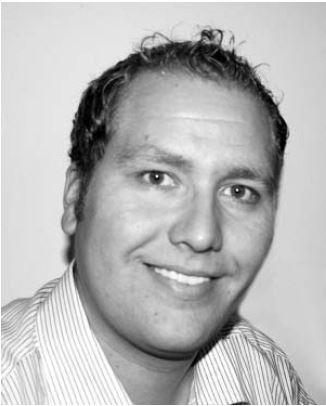
\includegraphics[width=1in,height=1.25in,clip,keepaspectratio]{ME.JPG}}]{Markus Enzweiler}
received the MSc degree in
computer science from the University of Ulm,
Germany, in 2005. Since 2006, he has been
working toward the PhD degree with the Image
and Pattern Analysis Group at the University of
Heidelberg, Germany, while on site at Daimler
Research in Ulm, Germany. In 2002 and 2003,
he was a visiting student researcher at the
Centre for Vision Research at York University,
Toronto, Canada. His current research focuses
on statistical models of human appearance with application to
pedestrian recognition in the domain of intelligent vehicles. He holds a
PhD scholarship from the Studienstiftung des deutschen Volkes
(German National Academic Foundation) and is an IEEE student
member. More details about his research and background can be found
at http://www.markus-enzweiler.de.
\end{IEEEbiography}
\begin{IEEEbiography}[{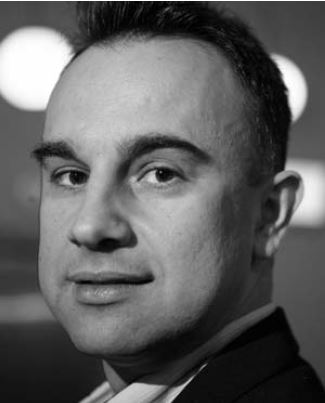
\includegraphics[width=1in,height=1.25in,clip,keepaspectratio]{DMG.JPG}}]{Dariu M. Gavrila}
received the MSc degree in
computer science from the Free University of
Amsterdam in 1990 and the PhD degree in
computer science from the University of Maryland
at College Park in 1996. Since 1997, he
has been a senior research scientist at Daimler
Research in Ulm, Germany. He was a visiting
researcher at the MIT Media Laboratory in
1996. In 2003, he became a professor in the
Faculty of Science at the University of Amsterdam,
chairing the area of Intelligent Perception Systems (part time).
Over the last decade, he has focused on visual systems for detecting
human presence and recognizing activity, with application to intelligent
vehicles and surveillance. He has published more than 20 papers in
this area and received the I/O Award 2007 from the Netherlands
Organization for Scientific Research (NWO). More details about his
research and background can be found at http://www.gavrila.net.
\end{IEEEbiography}
\end{document}
